% \iffalse meta-comment
%
% Copyright (C) 2012 Universite Laval
%
% This file may be distributed and/or modified under the conditions
% of the LaTeX Project Public License, either version 1.3c of this
% license or (at your option) any later version. The latest version
% of this license is in:
%
%   http://www.latex-project.org/lppl.txt
%
% and version 1.3c or later is part of all distributions of LaTeX
% version 2006/05/20 or later.
%
% This work has the LPPL maintenance status `maintained'.
%
% The Current Maintainer of this work is Universite Laval
% <ulthese-dev@bibl.ulaval.ca>.
%
% This work consists of the files ulthese.dtx and ulthese.ins
% and the derived files listed in the README file.
%
% \fi
%
% \iffalse
%<*dtx>
\ProvidesFile{ulthese.dtx}
%</dtx>
%<class>\NeedsTeXFormat{LaTeX2e}[2009/09/24]
%<class>\ProvidesClass{ulthese}%
%<*class>
  [2012/09/30 v1.0 Classe pour les theses et memoires de l'Universite Laval]
%</class>
%<*driver>
\documentclass[11pt]{ltxdoc}
  \usepackage[utf8]{inputenc}
  \usepackage[T1]{fontenc}
  \usepackage{natbib}
  \usepackage[francais]{babel}
  \usepackage[autolanguage]{numprint}
  \usepackage{mathpazo}
  \usepackage[scaled=0.92]{helvet}
  \usepackage{color,booktabs}
  \EnableCrossrefs
  \CodelineIndex
  \RecordChanges

  \definecolor{doclinkcolor}{rgb}{0,0,0.5}

  \usepackage{hyperref}
  \hypersetup{colorlinks,allcolors=doclinkcolor}

  \frenchbsetup{%
    CompactItemize=false,         % ne pas compacter les listes
    ThinSpaceInFrenchNumbers=true % espace fine dans les nombres
  }
\begin{document}
  \DocInput{ulthese.dtx}
\end{document}
%</driver>
% \fi
% \CheckSum{568}
% \DoNotIndex{\',\^,\`,\ ,\ae}
% \DoNotIndex{\RequirePackage,\ExecuteOptions,\ifthenelse,\ProcessOptions}
% \DoNotIndex{\newcommand,\newcommand*,\newboolean}
% \DoNotIndex{\setlength,\setboolean}
% \changes{1.0}{2012-09-30}{Version initiale}
% \GetFileInfo{ulthese.dtx}
% \title{\textsf{ulthese}: une classe pour les thèses et mémoires de
%   l'Université Laval\thanks{Ce document décrit la classe
%   \textsf{ulthese}~\fileversion, datée du \filedate.}}
% \author{Faculté des études supérieures et postdoctorales\thanks{%
%   Cette classe et sa documentation ont été rédigés par Vincent
%   Goulet~(Faculté des sciences et de génie) avec la collaboration de
%   Koassi D'Almeida~(Faculté des études supérieures et postdoctorales) et
%   Pierre Lasou~(Bibliothèque).}}
% \maketitle
% \tableofcontents
%
% \section{Introduction}
%
% La classe \textsf{ulthese} permet de composer avec {\LaTeX} des thèses
% et mémoires immédiatement conformes aux règles générales de
% présentation matérielle de la Faculté des études supérieures et
% postdoctorales (FESP) de l'Université Laval. Ces règles définissent
% principalement la présentation de la page titre des thèses et mémoires
% ainsi que la disposition du texte sur la page. La classe en elle-même
% est donc relativement simple.
%
% Cependant, la classe \textsf{ulthese} est basée sur la classe
% \textsf{memoir}, une extension de la classe standard \textsf{book}
% facilitant à plusieurs égards la préparation de documents d'allure
% professionnelle dans {\LaTeX}. La classe \textsf{memoir} est très
% configurable et incorpore d'office plus de 30 des paquetages
% (\emph{packages}) les plus populaires\footnote{%
%   Consulter la section~18.24 de la documentation de \textsf{memoir}
%   pour la liste ou encore le fichier journal (\emph{log}) de la
%   compilation d'un document utilisant la classe \textsf{ulthese}.}. %
% L'intégralité des fonctionnalités de \textsf{memoir} est disponible
% dans \textsf{ulthese}.
%
% La classe \textsf{memoir} fait maintenant partie des distributions
% {\LaTeX} modernes; elle devrait donc être installée et disponible sur
% votre système. La classe est livrée avec une documentation exhaustive:
% le manuel d'instructions fait près de 600~pages! Il peut être utile de
% s'y référer de temps à autre pour réaliser une mise en page
% particulière. Rechercher sur votre système le fichier |memman.pdf| ou
% le %
% \href{http://mirrors.ctan.org/macros/latex/contrib/memoir/memman.pdf}{%
%   consulter en ligne} %
% sur le site %
% \href{http://www.ctan.org/}{%
%   \emph{Comprehensive R Archive Network} (CTAN)}.
%
%
% \section{Installation}
%
% L'installation de la classe consiste à créer le fichier
% |ulthese.cls| et plusieurs gabarits |.tex| à partir du code source
% documenté se trouvant dans le fichier |ulthese.dtx|. Il est
% recommandé de simplement créer ces fichiers dans le dossier de
% travail de la thèse ou du mémoire.
%
% Pour procéder à l'installation, décompresser l'archive |ulthese.zip|
% dans le dossier de travail, puis compiler avec {\LaTeX} le fichier
% |ulthese.ins| en exécutant
% \begin{quote}
%   |latex ulthese.ins|
% \end{quote}
% depuis une invite de commande. Si l'on est peu familier avec
% l'invite de commande, on peut aussi procéder comme avec tout
% document {\LaTeX}, soit ouvrir le fichier |ulthese.ins| dans son
% éditeur de texte favori et lancer la compilation avec {\LaTeX},
% pdf{\TeX} ou pdf{\LaTeX} depuis celui-ci.
%
% \section{Utilisation}
%
% La classe est chargée avec la commande
% \begin{quote}
%   |\documentclass[|\meta{options}|]{ulthese}|
% \end{quote}
% Les marges, l'interligne et la numérotation des pages sont adaptées
% aux règles de présentation matérielle de la FESP. Les options et les
% commandes définies par la classe sont décrites dans les sections
% suivantes.
%
% \subsection{Options de la classe}
% \label{sec:utilisation:options}
%
% Les \meta{options} que l'on peut spécifier au chargement de la classe
% sont les suivantes:
% \begin{description}
% \item[|10pt|] sélectionne une taille de police de 10~points;
% \item[|11pt|] sélectionne une taille de police de 11~points;
% \item[|12pt|] sélectionne une taille de police de 12~points;
% \item[|nonatbib|] empêche de charger le paquetage \textsf{natbib} (voir
%   la section~\ref{sec:bibliographystyle});
% \item[|english, francais, ...|] langues utilisées dans le document;
% \item[\mdseries\meta{options memoir}] autres options du paquetage
%   \textsf{memoir}.
% \end{description}
%
% Si aucune taille de police n'est précisée, la classe utilisera une
% taille par défaut de 11~points. La taille des polices de la page
% titre n'est pas affectée par les options |10pt|, |11pt| et |12pt|.
%
% Le paquetage \textsf{natbib} est normalement chargé par la classe.
% L'option |nonatbib| permet d'empêcher le chargement en cas de
% conflit avec un autre paquetage de mise en forme de la
% bibliographie.
%
% Les langues sont passées au paquetage \textsf{babel}; voir la
% section~\ref{sec:langues}. Leur libellé devrait donc correspondre
% aux options de ce paquetage. La dernière langue spécifiée est la
% langue active par défaut dans le document.
%
% Toute autre option sera passée à la classe \textsf{memoir} dont,
% entre autres, le format du papier. Le format lettre nord-américain
% (option |letterpaper|) est utilisé par défaut. Si la thèse doit être
% imprimée en format international A4, utiliser l'option |a4paper|. La
% classe \textsf{memoir} est toujours chargée avec les options
% |twoside|, et |openright|.
%
% \subsection{Nouvelles commandes}
%
% La classe \textsf{ulthese} définit quelques nouvelles commandes
% servant principalement à créer la page titre et des éléments des pages
% liminaires.
%
% \subsubsection{Commandes de la page titre}
% \label{sec:commandes-pagetitre}
%
% Les commandes ci-dessous servent à définir les divers éléments de la
% page titre et leur disposition sur la page.
%
% \begin{DescribeMacro}{\titre}
%   Titre principal de la thèse ou du mémoire. Ne pas utiliser la
%   commande |\title| de {\LaTeX} pour ce faire.
%
%   Un titre très long devra être coupé manuellement avec |\\| ou
%   |\newline|. Dans un tel cas, il est également nécessaire de
%   retrancher de l'espacement vertical pour éviter que les autres
%   éléments de la page titre ne soient poussés vers le bas. Pour ce
%   faire, ajouter la déclaration
%   \begin{quote}
%     |\vspace*{-|$n$|\baselineskip}|
%   \end{quote}
%   à la fin de la \emph{dernière} ligne de titre s'il y a $n + 1$
%   lignes de titre au total.
%
%   Par exemple, la déclaration d'un titre d'une seule ligne est:
%   \begin{quote}
%     |\titre{Ceci est un titre d'une seule ligne}|
%   \end{quote}
%   Pour un titre de deux lignes, on écrira:
%   \begin{quote}
%     |\titre{Ceci est la première ligne d'un long titre \\| \\
%     |       et ceci est la seconde \vspace*{-1\baselineskip}}|
%   \end{quote}
%   Pour un titre de trois lignes, c'est alors:
%   \begin{quote}
%     |\titre{Ceci est la première ligne d'un très long titre \\| \\
%     |       pour lequel deux lignes ne suffisent pas \\| \\
%     |       alors voici la troisième \vspace*{-2\baselineskip}}|
%   \end{quote}
%   Ainsi de suite.
% \end{DescribeMacro}
%
% \begin{DescribeMacro}{\soustitre}
%   Sous-titre de la thèse ou du mémoire, le cas échéant. Les remarques
%   sur un long titre principal s'appliquent également au sous-titre.
% \end{DescribeMacro}
%
% \begin{DescribeMacro}{\auteur}
%   Nom complet de l'auteur de la thèse ou du mémoire, sous la forme
%   |Prénom Nom| avec seulement des majuscules initiales. Ne pas
%   utiliser la commande |\author| de {\LaTeX} pour le nom de l'auteur.
% \end{DescribeMacro}
%
% \begin{DescribeMacro}{\annee}
%   Année du dépôt final de la thèse ou du mémoire.
% \end{DescribeMacro}
%
% \begin{DescribeMacro}{\programme}
%   Nom du complet officiel du programme d'études comme «Doctorat en
%   informatique» ou «Maîtrise en mathématiques». Si le programme
%   comporte une majeure, séparer sa mention de celle du programme
%   principal par un tiret demi-quadratin (obtenu avec |--|).
% \end{DescribeMacro}
%
% \begin{DescribeMacro}{\PhD,}
%   \begin{DescribeMacro}{\MSc,}
%     \begin{DescribeMacro}{\MA, \dots}
%       Déclaration du type de grade auquel donne droit la thèse ou le
%       mémoire. Consulter le tableau~\ref{tab:grades} pour la liste
%       complète des commandes et des grades correspondants.
%     \end{DescribeMacro}
%   \end{DescribeMacro}
% \end{DescribeMacro}
%
% \begin{table}
%   \centering
%   \begin{tabular}{lp{9cm}}
%     \toprule
%     Commande & Nom du grade (sigle) \\
%     \midrule
%     |\LLD|\index{LLD=\verb+\LLD+}
%       & Docteur en droit (L.L.D.) \\
%     |\DPsy|\index{DPsy=\verb+\DPsy+}
%       & Docteur en psychologie (D.Psy.) \\
%     |\DThP|\index{DThP=\verb+\DThP+}
%       & Docteur en théologie pratique (D.Th.P.) \\
%     |\PhD|\index{PhD=\verb+\PhD+}
%       & Philosophi{\ae} doctor (Ph.D.) \\
%     \addlinespace[6pt]
%     |\LLM|\index{LLM=\verb+\LLM+}
%       & Maître en droit (L.L.M.) \\
%     |\MA|\index{MA=\verb+\MA+}
%       & Maître ès arts (M.A.) \\
%     |\MMus|\index{MMus=\verb+\MMus+}
%       & Maître en musique (M.Mus.) \\
%     |\MSc|\index{MSc=\verb+\MSc+}
%       & Maître ès sciences (M.Sc.) \\
%     |\MServSoc|\index{MServSoc=\verb+\MServSoc+}
%       & Maître en service social (M.Serv.Soc.) \\
%     |\MScGeogr|\index{MScGeogr=\verb+\MScGeogr+}
%       & Maître en sciences géographiques (M.Sc.G\'eogr.) \\
%     |\MATDR|\index{MATDR=\verb+\MATDR+}
%       & Maître en aménagement du territoire et développement régional
%       (M.ATDR) \\
%     \bottomrule
%   \end{tabular}
%   \caption{Commandes de déclaration du grade et libellés correspondants}
%   \label{tab:grades}
% \end{table}
%
% \begin{DescribeMacro}{\multifacultaire}
%   Déclaration d'une thèse ou d'un mémoire multifacultaire. Requiert
%   d'utiliser aussi la commande |\faculteUL| ci-dessous.
% \end{DescribeMacro}
%
% \begin{DescribeMacro}{\cotutelle}
%   Déclaration d'une thèse ou d'un mémoire réalisé en cotutelle avec
%   une autre université. Requiert d'utiliser aussi les commandes
%   |\univcotutelle| et |\gradecotutelle| ci-dessous.
% \end{DescribeMacro}
%
% \begin{DescribeMacro}{\univcotutelle}
%   Nom, ville et pays de l'université de cotutelle, déclarés sous la
%   forme
%   \begin{quote}
%     |\univcotutelle{Nom de l'université \\ Ville, Pays}|
%   \end{quote}
% \end{DescribeMacro}
%
% \begin{DescribeMacro}{\gradecotutelle}
%   Grade conféré par l'université de cotutelle, déclaré sous la forme
%   \begin{quote}
%     |\gradecotutelle{Nom du grade (sigle)}|
%   \end{quote}
% \end{DescribeMacro}
%
% \begin{DescribeMacro}{\extensionUdeS}
%   Déclaration que la thèse est réalisée en extension à l'Université
%   de Sherbrooke. Requiert d'utiliser aussi les commandes
%   |\faculteUL| et |\faculteUdeS| ci-dessous.
% \end{DescribeMacro}
%
% \begin{DescribeMacro}{\extensionUQO}
%   Déclaration que la thèse est réalisée en extension à l'Université du
%   Québec en Outaouais. Requiert d'utiliser aussi les commandes
%   |\faculteUL| et |\faculteUQO| ci-dessous.
% \end{DescribeMacro}
%
% \begin{DescribeMacro}{\extensionUQAC}
%   Déclaration que le mémoire est réalisé en extension à l'Université
%   du Québec à Chicoutimi. Requiert d'utiliser aussi les commandes
%   |\faculteUL| et |\faculteUQAC| ci-dessous.
% \end{DescribeMacro}
%
% \begin{DescribeMacro}{\faculteUL}
%   Cette macro a deux usages:
%   \begin{enumerate}
%   \item noms des facultés pour les thèses et mémoires
%     multifacultaires, séparés par des commandes |\\|;
%   \item nom de la faculté de l'Université Laval où sont réalisés les
%     thèses et mémoires en extension aux universités de Sherbrooke, du
%     Québec en Outaouais ou du Québec à Chicoutimi.
%   \end{enumerate}
% \end{DescribeMacro}
%
% \begin{DescribeMacro}{\faculteUdeS}
%   Nom de la faculté de l'Université de Sherbrooke hébergeant la thèse
%   en extension.
% \end{DescribeMacro}
%
% \begin{DescribeMacro}{\faculteUQO}
%   Nom de la faculté de l'Université du Québec en Outaouais hébergeant
%   la thèse en extension.
% \end{DescribeMacro}
%
% \begin{DescribeMacro}{\faculteUQAC}
%   Nom de la faculté de l'Université du Québec à Chicoutimi hébergeant
%   le mémoire en extension.
% \end{DescribeMacro}
%
% \begin{DescribeMacro}{\pagetitre}
%   Déclaration de création de la page titre. Ne pas utiliser la
%   commande |\pagetitle| de {\LaTeX} pour ce faire. De toutes les
%   commandes ci-dessus, c'est la seule qui doit se trouver dans le
%   corps du document plutôt que dans le préambule.
% \end{DescribeMacro}
%
% \subsubsection{Commandes des pages liminaires}
%
% La classe définit deux commandes pour créer des pages liminaires
% prévues aux règles de présentation matérielle.
%
% \begin{DescribeMacro}{\dedicace}
%   La commande |\dedicace| ajoute une dédicace («À mes parents», «À
%   Camille») à la thèse ou au mémoire. La dédicace est disposée seule
%   sur une page recto, à une dizaine de lignes de la marge du haut et
%   alignée à droite. Par défaut, elle est composée en italique.
% \end{DescribeMacro}
%
% \begin{DescribeMacro}{\epigraphe}
%   La commande |\epigraph| sert à ajouter une épigraphe au début du
%   document. Comme la dédicace, l'épigraphe est disposée seule sur une
%   page recto, à une dizaine de lignes de la marge du haut et alignée à
%   droite. La commande accepte deux arguments, soit le texte de la
%   citation et son auteur ou la source, dans l'ordre.
% \end{DescribeMacro}
%
% Pour ajouter une épigraphe au début d'un ou plusieurs chapitres,
% utiliser directement la commande |\epigraph| de \textsf{memoir}, sur
% laquelle |\dedicace| et |\epigraphe| sont d'ailleurs basées.
%
% \subsection{Citations}
% \label{sec:citations}
%
% \begin{DescribeEnv}{quote}
%   {\LaTeX} offre deux environnements pour les citations dans le
%   texte: |quote| et |quotation|. Le premier sert pour les citations
%   «courtes», quelques lignes au plus. Dans la classe, le texte est
%   alors placé en retrait des marges normales de 10~mm à gauche et à
%   droite.
% \end{DescribeEnv}
%
% \begin{DescribeEnv}{quotation}
%   L'environnement |quotation|, quant à lui, doit être utilisé pour
%   les citations «longues», celles qui peuvent s'étendre sur plus de
%   cinq lignes ou, surtout, plus d'un paragraphe. Dans la classe, le
%   texte est alors toujours placé en retrait de 10~mm, mais également
%   à interligne simple. De plus, les paragraphes, le cas échéant,
%   sont séparés d'un espace vertical afin de bien les distinguer les
%   uns des autres.
% \end{DescribeEnv}
%
% \subsection{Interligne}
%
% \begin{DescribeMacro}{\OnehalfSpacing}
%   L'espacement d'un interligne et demi utilisé dans la classe est
%   obtenu avec la commande |\OnehalfSpacing| de \textsf{memoir}.
%   L'interligne simple est automatiquement rétabli pour la page
%   titre, la table des matières, la liste des tableaux, la liste
%   des figures et les longues citations (section~\ref{sec:citations}).
% \end{DescribeMacro}
%
% \begin{DescribeMacro}{\SingleSpacing}
%   Si ce devait être nécessaire ailleurs dans le document, la
%   commande |\SingleSpacing| permet de passer à l'interligne simple.
% \end{DescribeMacro}
%
%
% \subsection{Autres paquetages chargés}
% \label{sec:paquetages}
%
% Outre \textsf{memoir} et \textsf{babel}, la classe \textsf{ulthese}
% charge pour son usage quelques paquetages qui peuvent aussi être
% utiles pour l'utilisateur de la classe. Il n'est donc pas nécessaire
% de charger de nouveau les paquetages suivants:
% \begin{description}
% \item[\normalfont\textsf{natbib}] gestion de la bibliographie (si
%   l'option |nonatbib| de la classe est absente; voir aussi la
%   section~\ref{sec:bibliographystyle});
% \item[\normalfont\textsf{numprint}] permet de composer
%   automatiquement des nombres avec un séparateur toutes les trois
%   positions (une espace en français). Requis par la commande
%   |\nombre| de \textsf{babel};
% \item[\normalfont\textsf{graphicx}] support pour l'insertion et la
%   manipulation de graphiques;
% \item[\normalfont\textsf{xcolor}] extension du paquetage
%   \textsf{color} pour gérer les couleurs dans le texte;
% \item[\normalfont\textsf{textcomp}] multitude de symboles spéciaux,
%   dont un beau symbole de copyright, \textcopyright.
% \item[\normalfont\textsf{helvet}] remplacement de la police sans
%   empattements (\emph{serifs}) standard par la police Helvetica pour
%   composer la page titre. Le paquetage est chargé avec l'option
%   |scaled=0.92|. Consulter la section~\ref{sec:police} pour des
%   informations additionnelles.
% \end{description}
% La section~\ref{sec:meo} sur la mise en {\oe}uvre de la classe
% fournit plus de détails sur la liste des paquetages chargés et les
% raisons pour lesquelles ils sont requis dans la classe.
%
% \section{Français et autres langues}
% \label{sec:langues}
%
% Une complication additionnelle pour les auteurs rédigeant dans une
% langue autre que l'anglais consiste à adapter {\LaTeX} à leur
% langue, qu'il s'agisse des mots clés, de la typographie ou de la
% césure des mots. La solution à ce problème provient du paquetage
% standard \textsf{babel}. Celui-ci permet de combiner plusieurs
% langues dans un même document et de passer de l'une à l'autre
% facilement. Il est chargé par la classe \textsf{ulthese}.
%
% Aucune langue n'est spécifiée dans la classe. La plupart des auteurs
% auront recours à l'anglais et au français, ne serait-ce que pour les
% deux résumés demandés par la FESP. Les langues utilisées dans le
% document doivent être spécifiées comme options à la classe, tel que
% mentionné à la section~\ref{sec:utilisation:options}. La
% \emph{dernière} langue spécifiée devient par défaut la langue active
% du document.
%
% \begin{DescribeMacro}{\selectlanguage}
%   La commande |\selectlanguage| de \textsf{babel} permet de passer de
%   la langue courante à la langue spécifiée en argument.
% \end{DescribeMacro}
%
% \begin{DescribeEnv}{otherlanguage}
%   L'environnement |otherlanguage| de \textsf{babel} permet de faire
%   la même chose que la commande |\selectlanguage|, sauf que le
%   changement de langue est local à l'environnement --- utile pour
%   les brefs changements de langue.
% \end{DescribeEnv}
%
% Si vous n'êtes pas autrement familier avec le paquetage \textsf{babel},
% consulter sa documentation, ne serait-ce que les chapitres consacrés
% aux langues utilisées dans votre thèse ou mémoire. Rechercher sur
% votre système le fichier |babel.pdf| ou le %
% \href{http://mirrors.ctan.org/macros/latex/required/babel/babel.pdf}{%
%   consulter en ligne} %
% sur CTAN.
%
% \section{Police de caractère du document}
% \label{sec:police}
%
% Les documents {\LaTeX} sont facilement reconnaissables par leur
% police de caractère par défaut, Computer Modern. Avec toute
% distribution {\LaTeX} moderne, il est maintenant simple d'utiliser
% l'une ou l'autre des polices Postscript standards. D'ailleurs la
% classe \textsf{ulthese} utilise la police sans empattements
% Helvetica pour composer la page titre.
%
% La FESP permet l'utilisation des polices Times et
% Palatino\footnote{%
%   Police utilisée dans le présent document.} %
% dans les thèse et mémoires {\LaTeX}. Pour utiliser ces polices,
% charger les paquetages \textsf{mathptmx} ou \textsf{mathpazo},
% respectivement. Pour les détails, consulter la documentation de
% l'ensemble de paquetages PSNFSS. Rechercher sur votre système le
% fichier |psnfss2e.pdf| ou le %
% \href{http://mirrors.ctan.org/macros/latex/required/psnfss/psnfss2e.pdf}{%
% consulter en ligne} %
% sur CTAN.
%
% \section{Gabarits}
%
% Il est recommandé de segmenter tout document d'une certaine ampleur
% dans des fichiers |.tex| distincts pour chaque partie ---
% habituellement un fichier par chapitre. Le document complet est
% composé à l'aide d'un fichier maître qui contient le préambule
% {\LaTeX} et un ensemble de commandes
% |\include|\index{include=\verb+\include+} pour réunir les parties
% dans un tout.
%
% La classe \textsf{ulthese} est livrée avec un ensemble de gabarits sur
% lesquels se baser pour:
% \begin{itemize}
% \item les fichiers maîtres de divers types de thèses et mémoires
%   (standard, sur mesure, en cotutelle, en extension, etc.);
% \item les fichiers des parties les plus usuelles (résumés français
%   et anglais, avant-propos, introduction, chapitres, conclusion,
%   etc.).
% \end{itemize}
% Les noms des fichiers devraient permettre de facilement identifier
% leur contenu (une bonne pratique; |rappels.tex| est plus parlant et
% résiste mieux aux changements à l'ordre des chapitres que
% |chapitre1.tex|).
%
% Pour débuter la rédaction, renommer le gabarit de document maître
% approprié d'après votre numéro de dossier. Par exemple, l'étudiante
% dont le numéro de dossier est 900352789 et qui entame la rédaction
% d'une thèse multifacultaire renommera le fichier
% \begin{quote}
%   |gabarit-doctorat-multifacultaire.tex|
% \end{quote}
% en
% \begin{quote}
%   |900352789.tex|.
% \end{quote}
% Les autres gabarits de documents maîtres peuvent alors être
% supprimés.
%
% Les gabarits comportent des commentaires succincts pour vous guider
% dans la préparation de votre document. Les sections suivantes
% fournissent des détails additionnels, et ce, dans l'ordre où les
% commandes apparaissent dans les gabarits.
%
% \subsection{Encodage des fichiers}
%
% Taper de longs textes en français en {\LaTeX} devient rapidement
% pénible si on utilise les commandes |\'e|, |\`a| ou |\^e| pour entrer
% les lettres accentuées. Afin de pouvoir plutôt entrer directement |é|,
% |à| ou |ê|, {\LaTeX} doit être configuré pour reconnaître les lettres
% accentuées. C'est le rôle du paquetage \textsf{inputenc}.
%
% Cependant, il existe plusieurs manières différentes d'encoder --- ou
% d'enregistrer --- les lettres accentuées et autres caractères
% spéciaux (comme, par exemple, le symbole de l'euro) dans un
% ordinateur. La méthode la plus répandue et celle standard sur les
% versions récentes des systèmes d'exploitation Linux et OS~X est
% l'UTF-8 de la norme
% \href{http://fr.wikipedia.org/wiki/Unicode}{Unicode}. Les gabarits
% sont livrés dans ce type d'encodage.
%
% La déclaration
% \begin{quote}
%   |\usepackage[utf8]{inputenc}|
% \end{quote}
% dans le préambule assure que {\LaTeX} traitera correctement des
% fichiers source encodés en UTF-8.
%
% La norme Unicode n'est pas aussi uniformément supportée par Windows.
% Selon l'éditeur de texte employé et la version du système
% d'exploitation, il peut être nécessaire d'utiliser les normes
% d'encodage %
% \href{http://fr.wikipedia.org/wiki/ISO_8859-1}{ISO~8859-1} %
% (ou Latin-1; option |latin1| de \textsf{inputenc}), %
% \href{http://fr.wikipedia.org/wiki/ISO_8859-15}{ISO~8859-15} %
% (ou Latin-9; option |latin9|) ou %
% \href{http://fr.wikipedia.org/wiki/Windows-1252}{Windows-1252} %
% (options |cp1252| ou |ansinew|).
%
%
% \subsection{Paquetages additionnels}
%
% Tel qu'explicité à la section~\ref{sec:paquetages}, la classe
% charge déjà quelques paquetages. Cependant, il est fort probable que
% vous devrez en charger d'autres pour composer votre document. Les
% gabarits prévoient un endroit pour le chargement de paquetages
% additionnels. Il est recommandé d'inscrire vos commandes
% |\usepackage| à cet endroit afin de respecter un certain ordre de
% chargement; voir la section suivante.
%
% Si vous utilisez un paquetage non standard dans les distributions
% courantes (MiK\TeX, \TeX~Live, Mac\TeX), vous devez le fournir avec
% le code source de votre document lors du dépôt final.
%
% \subsection{Hyperliens}
% \label{sec:hyperref}
%
% Le paquetage \textsf{hyperref} permet de transformer toutes les
% références en hyperliens cliquables lorsque le document {\LaTeX} est
% produit avec |pdflatex|. L'interaction de ce paquetage avec les autres
% est parfois (voire souvent) délicate. Pour cette raison, il est
% habituellement nécessaire de charger \textsf{hyperref} en tout
% dernier. C'est pourquoi il n'est pas chargé dans la classe, mais
% plutôt dans les gabarits. Prendre soin de maintenir le dernier rang de
% chargement lors de l'édition d'un gabarit.
%
% La configuration du paquetage dans les gabarits fait en sorte que
% les liens sont simplement signalés par une couleur de texte
% légèrement contrastante. L'utilisation de couleurs dans un document
% requiert le paquetage |xcolor|, chargé par la classe. La couleur de
% lien par défaut, |ULlinkcolor|, est définie dans la classe; voir la
% section~\ref{sec:couleurs}.
%
% \subsection{Police sans empattements}
%
% Tel que mentionné à la section~\ref{sec:police}, la police sans
% empattements Helvetica est chargée par la classe pour composer la page
% titre. Ainsi, toute utilisation des commandes |\textsf| et |\sffamily|
% sélectionnera cette police.
%
% Si vous composez la thèse ou le mémoire dans la police par défaut de
% {\LaTeX}, vous souhaiterez sans doute que les commandes ci-dessus
% sélectionnent plutôt la version sans empattements de Computer
% Modern; comparer
% \begin{quote}
%   \sffamily Texte sans empattements en Helvetica
% \end{quote}
% et
% \begin{quote}
%   \fontfamily{cmss}\selectfont Texte sans empattements en Computer Modern
% \end{quote}
% Pour ce faire, décommentez la ligne du gabarit afin que la
% commande
% \begin{quote}
%   |\renewcommand{\sfdefault}{cmss}|
% \end{quote}
% apparaisse dans le préambule.
%
% \subsection{Options de \textsf{babel}}
%
% \begin{DescribeMacro}{\frenchbsetup}
%   La commande |\frenchbsetup|\index{frenchbsetup=\verb+\frenchbsetup+}
%   de \textsf{babel} permet de contrôler certains ajustements
%   typographiques apportés par le paquetage en mode français. Consulter
%   la documentation de \textsf{babel} pour la liste des options de
%   configuration disponibles.
% \end{DescribeMacro}
%
% Les concepteurs de la classe \textsf{ulthese}  proposent deux
% ajustements dans les gabarits:
% \begin{enumerate}
% \item l'option |CompactItemize=false| évite que le mode français de
%   \textsf{babel} ne diminue l'espacement vertical dans les listes;
% \item avec l'option |ThinSpaceInFrenchNumbers=true|, une espace fine
%   sera utilisée comme séparateur des milliers dans les nombres plutôt
%   qu'une espace pleine.
% \end{enumerate}
% \begin{DescribeMacro}{\nombre}
%   D'ailleurs, à ce sujet, le paquetage \textsf{numprint} étant
%   chargé dans la classe, on peut utiliser la commande |\nombre| pour
%   formater automatiquement les nombres. Par exemple, le résultat de
%   |\nombre{123456789}| est \nombre{123456789}.
% \end{DescribeMacro}
%
% \subsection{Style de la bibliographie}
% \label{sec:bibliographystyle}
%
% \begin{DescribeMacro}{\bibliographystyle}
%   Il est fortement recommandé d'utiliser BIB{\TeX} pour la préparation
%   de la bibliographie. Le formatage de la bibliographie est contrôlé
%   par un style choisi par la commande |\bibliographystyle|. Les styles
%   standards de {\LaTeX} sont |plain|, |unsrt|, |alpha| et |abbrv|.
% \end{DescribeMacro}
%
% Pour plus de flexibilité, il est recommandé d'utiliser le paquetage
% \textsf{natbib} pour la gestion des références et des styles de la
% bibliographie. Entre autres choses, ce paquetage supporte le style de
% citation auteur-année fréquemment employé en sciences naturelles,
% plusieurs commandes de citation, un grand nombres de styles de
% bibliographie ainsi que des entrées spécifiques pour les numéros ISBN
% et les URL. Le paquetage fournit des styles de bibliographie
% |plainnat|, |unsrtnat| et |abbrvnat| similaires aux styles standards,
% mais plus complets. Il existe des
% \href{http://mirrors.ctan.org/biblio/bibtex/contrib/bib-fr/}{versions
%   francisées} de ces styles (et de quelques autres) dans CTAN.
%
% Afin d'assurer le bon fonctionnement avec \textsf{babel}, le
% paquetage \textsf{natbib} est chargé par la classe \textsf{ulthese}
% (à moins que l'option |nonatbib| ne soit spécifiée). Pour consulter
% sa documentation, rechercher sur votre système le fichier
% |natbib.pdf| ou le %
% \href{http://mirrors.ctan.org/macros/latex/contrib/natbib/natbib.pdf}{%
%   consulter en ligne} %
% sur CTAN.
%
% De plus, Vincent Goulet a préparé la feuille de style
% |francais.bst| compatible avec \textsf{natbib}; consulter la
% section \href{http://vgoulet.act.ulaval.ca/latex/}{LaTeX en
% français} de son site Web. La feuille de style permet de composer
% des bibliographies auteur-année respectant les normes de typographie
% française telles qu'édictées dans \cite{Malo:1996}. Pour utiliser ce
% style, on spécifera dans le préambule du document LaTeX
% \begin{quote}
%   |\bibliographystyle{francais}|
% \end{quote}
%
% Autrement, la FESP n'a pas d'exigences particulières quant à la
% présentation de la bibliographie (présentation du titre, des auteurs
% et autres informations bibliographiques).
%
% \subsection{Déclarations de la page titre}
%
% Les gabarits comportent toutes les déclarations nécessaires pour
% composer la page titre des divers types de thèse ou de mémoires.
% Vous devez remplacer les éléments se trouvant entre crochets <~> en
% respectant la forme indiquée. Assurez-vous de supprimer les
% caractères < et > afin qu'il n'apparaissent pas sur la page titre de
% votre document.
%
% \subsection{Pages liminaires}
%
% \begin{DescribeMacro}{\frontmatter}
%   La commande |\frontmatter| déclare que {\LaTeX} doit considérer le
%   matériel qui suit comme des pages liminaires. En pratique, cela
%   résulte essentiellement en une numérotation des pages en chiffres
%   romains.
% \end{DescribeMacro}
%
% Les normes de présentation de la FESP édictent que les thèses et
% mémoires devraient comporter les pages liminaires suivantes, dans
% l'ordre:
% \begin{enumerate}
% \item la page titre (obligatoire);
% \item un résumé en français (obligatoire);
% \item un résumé en anglais (recommandé mais non obligatoire);
% \item une table des matières (obligatoire);
% \item une liste des tableaux;
% \item une liste des figures;
% \item une liste des abbréviations et des sigles;
% \item une dédicace;
% \item une épigraphe;
% \item des remerciements;
% \item un avant-propos (obligatoire dans le cas d'un mémoire ou d'une
%   thèse avec insertion d'articles).
% \end{enumerate}
%
% Les commandes
% \begin{quote}
%   |\pagetitre| \\
%   |\tableofcontents| \\
%   |\listoftables| \\
%   |\listoffigures| \\
%   |\dedicace{|\meta{texte}|}| \\
%   |\epigraphe{|\meta{texte}|}{|\meta{auteur}|}|
% \end{quote}
% permettent de générer les pages correspondantes. Seules les deux
% dernières commandes admettent des arguments.
%
% \begin{DescribeMacro}{\chapter*}
%   Les résumés, la liste des abbréviations et des sigles, les
%   remerciements et l'avant-propos sont composés comme des chapitres
%   normaux, mais sans être numérotés. Il faut donc définir ces éléments
%   avec la commande |\chapter*|.
% \end{DescribeMacro}
%
% \begin{DescribeMacro}{\phantomsection}
%   \begin{DescribeMacro}{\addcontentsline}
%     Les sections declarées avec la commande |\chapter*|
%     n'apparaissent pas dans la table des matières. Comme les normes
%     de présentation de la FESP exigent que toutes les pages
%     liminaires y figurent, on fait suivre les commandes
%     |\chapter*{|\meta{Titre}|}| des commandes
%   \end{DescribeMacro}
% \end{DescribeMacro}
% \begin{quote}
%   |\phantomsection\addcontentsline{toc}{chapter}{|\meta{Titre}|}|
% \end{quote}
% Celles-ci ajoutent à la table des matières (|toc|) une section de
% niveau |chapter| dont le titre est \meta{Titre}. La commande
% |\phantomsection| est rendue nécessaire (ou recommandée) par le
% paquetage \textsf{hyperref}.
%
% \subsection{Corps du document}
%
% \begin{DescribeMacro}{\mainmatter}
%   La commande |\mainmatter| délimite le début du corps du document. La
%   numérotation des pages passe en chiffres arabes.
% \end{DescribeMacro}
%
% Le corps du document devrait normalement compter une introduction (non
% numérotée), un développement divisé en chapitres (numérotés) et une
% conclusion (non numérotée).
%
% \subsection{Annexes}
%
% \begin{DescribeMacro}{\appendix}
%   Si la thèse ou le mémoire comporte une ou plusieurs annexes,
%   composer celles-ci comme des chapitres normaux insérés dans le
%   document maître après la commande |\appendix|. Cette commande a
%   pour effet de passer d'un mode de numération numérique (1, 2, 3,
%   \dots) à un mode alphabétique (A, B, C, \dots).
% \end{DescribeMacro}
%
% \subsection{Bibliographie}
%
% \begin{DescribeMacro}{\bibliography}
%   Si vous utilisez BIB{\TeX}, la bibliographie est insérée dans le
%   document à l'endroit où apparait la commande |\bibliography| dans le
%   code source.
% \end{DescribeMacro}
%
% Consulter la section~\ref{sec:bibliographystyle} pour des
% informations additionnelles sur la préparation de la bibliographie.
%
% \section{Aide additionnelle}
%
% Pour obtenir de l'aide additionnelle sur l'utilisation de la classe
% \textsf{ulthese} (et sur celle de {\LaTeX} en général), prière de
% consulter d'abord
% \begin{enumerate}
% \item le \href{http://www.theses.ulaval.ca/wiki/}{WikiThèse} de
%   l'Université Laval;
% \item les
%   \href{http://listes.ulaval.ca/listserv/archives/ulthese-aide.html}{archives}
%   de la liste de distribution \texttt{ulthese-aide}.
% \end{enumerate}
% Si la réponse à votre question ne se trouve ni dans le wiki, ni dans
% les archives, alors écrire à l'adresse
% \href{mailto:ulthese-aide@bibl.ulaval.ca}{\url{ulthese-aide@bibl.ulaval.ca}}.
%
% \StopEventually{\PrintChanges\PrintIndex}
%
% ^^A Début du code de la classe
%
% \appendix
% \section{Mise en {\oe}uvre}
% \label{sec:meo}
%
% Cette section passe en revue le code {\TeX} et {\LaTeX} de la
% classe. Elle ne risque d'intéresser que les personnes qui souhaitent
% explorer comment la classe est programmée.
%
% \subsection{Options de la classe}
%
% Il y a deux options propres à la classe: la taille de la police de
% caractères en points et la possibilité d'empêcher le chargement du
% paquetage \textsf{natbib}.
%
% \begin{macro}{nonatbib}
%   Pour des raisons de programmation, on traite l'option |nonatbib|
%   en premier. Celle-ci permet d'empêcher la classe de charger le
%   paquetage \textsf{natbib} en cas d'incompatibilité avec d'autres
%   paquetages spécialisés de mise en forme de la bibliographie. Le
%   paquetage \textsf{ifthen} est nécessaire pour définir cette option
%   booléenne et pour plusieurs autres usages internes à la classe.
%    \begin{macrocode}
%<*class>
\RequirePackage{ifthen}
\newboolean{UL@natbib}
\setboolean{UL@natbib}{true}
\DeclareOption{nonatbib}{\setboolean{UL@natbib}{false}}
%    \end{macrocode}
% \end{macro}
%
% Les valeurs possibles pour la taille de la police de caractères sont
% |10pt|, |11pt| et |12pt|. Cette option est gérée au niveau de la
% classe afin de s'assurer que les divers éléments sur la page titre
% sont toujours de la même taille. La taille de la police par défaut
% permet de déterminer si, par exemple, le titre du document doit être
% dans la taille |\Huge|, |\huge| ou |\LARGE| de \textsf{memoir}.
%
% \begin{macro}{\UL@ptsize}
%   La taille de la police est passée à \textsf{memoir} et la macro
%   |\UL@ptsize| stocke la taille des caractères pour usage futur.
%    \begin{macrocode}
\newcommand*{\UL@ptsize}{}
\DeclareOption{10pt}{%
  \PassOptionsToClass{10pt}{memoir}
  \renewcommand*{\UL@ptsize}{10}}
\DeclareOption{11pt}{%
  \PassOptionsToClass{11pt}{memoir}
  \renewcommand*{\UL@ptsize}{11}}
\DeclareOption{12pt}{%
  \PassOptionsToClass{12pt}{memoir}
  \renewcommand*{\UL@ptsize}{12}}
%    \end{macrocode}
% \end{macro}
%
% \subsection{Chargement de la classe \textsf{memoir}}
%
% Toutes les options de la classe sont passées à \textsf{memoir}. Le
% format de papier et la taille de police par défaut sont, dans
% l'ordre, |letterpaper| et |11pt|. Les options de \textsf{memoir}
% |twoside| et |openright| sont explicitement déclarées afin d'éviter
% toute tentative de passer outre à ces exigences de la FESP.
%    \begin{macrocode}
\DeclareOption*{\PassOptionsToClass{\CurrentOption}{memoir}}
\ExecuteOptions{11pt,letterpaper}
\ProcessOptions
\LoadClass[twoside,openright]{memoir}
%    \end{macrocode}
%
% \subsection{Paquetages requis}
%
% La classe s'efforce de charger un minimum de paquetages afin d'éviter
% les conflits potentiels.
%
%  Il est aujourd'hui préférable d'utiliser les polices T1.
%    \begin{macrocode}
\RequirePackage[T1]{fontenc}
%    \end{macrocode}
%
% Le paquetage \textsf{natbib} doit être chargé avant \textsf{babel}
% pour bien fonctionner. C'est pourquoi il est chargé dans la classe,
% à moins que l'option |nonatbib| n'ait été spécifiée au chargement de
% la classe.
%    \begin{macrocode}
\ifthenelse{\boolean{UL@natbib}}{\RequirePackage{natbib}}{}
%    \end{macrocode}
%
% Le support pour les langues autres que l'anglais est offert par le
% paquetage \textsf{babel}. Les langues sont passées en option de la
% classe, et non du paquetage. Le paquetage \textsf{numprint} est
% requis par \textsf{babel} pour la définition de la commande de mise
% en forme des nombres |\nombre|.
%    \begin{macrocode}
\RequirePackage{babel}
\RequirePackage[autolanguage]{numprint}
%    \end{macrocode}
%
% L'insertion du logo de l'Université sur la page titre requiert
% \textsf{graphicx}. On définit également une couleur pour les
% hyperliens dans le document (mais \textsf{hyperref} est chargé dans
% les gabarits afin de demeurer le dernier paquetage chargé; voir la
% section~\ref{sec:hyperref}).
%    \begin{macrocode}
\RequirePackage{graphicx}
\RequirePackage{xcolor}
%    \end{macrocode}
%
% La commande |\textcopyright| utilisée sur la page titre requiert le
% paquetage \textsf{textcomp} pour obtenir un beau signe de copyright.
%    \begin{macrocode}
\RequirePackage{textcomp}
%    \end{macrocode}
%
% \subsection{Police pour la page titre}
%
% La page titre est composée dans la police Helvetica. Le chargement
% du paquetage \textsf{helvet} a pour effet de redéfinir la commande
% |\sfdefault|.
%    \begin{macrocode}
\RequirePackage[scaled=0.92]{helvet}
%    \end{macrocode}
%
% \subsection{Couleur des hyperliens}
% \label{sec:couleurs}
%
% La classe définit une couleur standard pour les hyperliens, une
% teinte de bleu assez foncée pour être à fois visible en couleur et
% peu contrastante si le document est imprimé en noir et blanc.
%    \begin{macrocode}
\definecolor{ULlinkcolor}{rgb}{0,0,0.3}
%    \end{macrocode}
%
% \subsection{Marges}
%
% Les marges exigées par les normes de présentation de la FESP sont de
% 25~mm partout, sauf 35~mm pour la marge de reliure (gauche pour les
% pages impaires, droite pour les pages paires). Le pied de page est
% placé de sorte que le folio de page se retrouve à 10~mm du bas de la
% page.
%    \begin{macrocode}
\setlrmarginsandblock{35mm}{25mm}{*}
\setulmarginsandblock{25mm}{*}{1}
\setheadfoot{\baselineskip}{20mm}
\checkandfixthelayout[lines]
%    \end{macrocode}
%
% \subsection{Interligne}
%
% L'espacement entre les lignes est d'un interligne et demi.
% L'espacement «double» entre les paragraphes est fixé à
% |0.5\baselineskip| afin d'en arriver à une disposition agréable à
% l'{\oe}il. Le retrait de première ligne est supprimé puisque plus
% nécessaire suite à l'ajout de l'espacement entre les paragraphes.
%    \begin{macrocode}
\OnehalfSpacing
\setlength{\parskip}{0.5\baselineskip}
\setlength{\parindent}{0em}
%    \end{macrocode}
%
% La table des matières, la liste des tableaux et la liste des figures
% sont composées à interligne simple.
%    \begin{macrocode}
\renewcommand{\tocheadstart}{\SingleSpacing\chapterheadstart}
\renewcommand{\lotheadstart}{\SingleSpacing\chapterheadstart}
\renewcommand{\lofheadstart}{\SingleSpacing\chapterheadstart}
%    \end{macrocode}
%
% \subsection{Entêtes et pieds de page}
%
% Les règles pour les entêtes et pieds de page sont uniformes pour
% tout le document: aucun entête et folio sur le bord extérieur du
% pied de page. On définit un style de page pour ce faire ainsi qu'un
% alias entre le nouveau style |ul| et le style standard |plain|.
% Raison: les premières pages de chapitres utilisent par défaut le
% style |plain|; avec l'alias c'est le style |ul| qui sera activé.
%    \begin{macrocode}
\makepagestyle{ul}
  \makeevenfoot{ul}{\thepage}{}{}
  \makeoddfoot{ul}{}{}{\thepage}
\aliaspagestyle{plain}{ul}
\pagestyle{ul}
%    \end{macrocode}
%
% \subsection{Page titre}
%
% La page titre est composée avec les polices présentées au
% tableau~\ref{tab:polices}. Les commandes sélectionnant ces polices
% sont adaptées selon la taille de police choisie pour le document
% afin d'être toujours identiques.
%
% \begin{table}
%   \centering
%   \begin{tabular}{ll}
%     \toprule
%     Élément          & Police \\
%     \midrule
%     Titre            & 20~points gras \\
%     Sous-titre       & 17~points gras \\
%     Auteur           & 14~points gras \\
%     Nom du programme & 14~points gras \\
%     Autres éléments  & 14~points normal \\
%     \bottomrule
%   \end{tabular}
%   \caption{Taille et type de police des éléments de la page titre}
%   \label{tab:polices}
% \end{table}
%
%    \begin{macrocode}
\ifthenelse{\UL@ptsize=10}{%
  \newcommand*{\UL@fonttitle}{\normalfont\Huge\bfseries\sffamily}
  \newcommand*{\UL@fontsubtitle}{\normalfont\huge\bfseries\sffamily}
  \newcommand*{\UL@fontauthor}{\normalfont\LARGE\bfseries\sffamily}
  \newcommand*{\UL@fontprogram}{\UL@fontauthor}
  \newcommand*{\UL@fontbase}{\normalfont\LARGE\sffamily}}{}
\ifthenelse{\UL@ptsize=11}{%
  \newcommand*{\UL@fonttitle}{\normalfont\huge\bfseries\sffamily}
  \newcommand*{\UL@fontsubtitle}{\normalfont\LARGE\bfseries\sffamily}
  \newcommand*{\UL@fontauthor}{\normalfont\Large\bfseries\sffamily}
  \newcommand*{\UL@fontprogram}{\UL@fontauthor}
  \newcommand*{\UL@fontbase}{\normalfont\Large\sffamily}}{}
\ifthenelse{\UL@ptsize=12}{%
  \newcommand*{\UL@fonttitle}{\normalfont\LARGE\bfseries\sffamily}
  \newcommand*{\UL@fontsubtitle}{\normalfont\Large\bfseries\sffamily}
  \newcommand*{\UL@fontauthor}{\normalfont\large\bfseries\sffamily}
  \newcommand*{\UL@fontprogram}{\UL@fontauthor}
  \newcommand*{\UL@fontbase}{\normalfont\large\sffamily}}{}
%    \end{macrocode}
%
% Définition de deux valeurs booléennes servant à adapter la
% composition de la page titre plus loin: y a-t-il un sous-titre ou
% non et est-ce que le type de programme (doctorat ou maîtrise) est
% masculin ou non?
%    \begin{macrocode}
\newboolean{UL@hassubtitle}
\newboolean{UL@isprogmasc}
%    \end{macrocode}
%
% Définition des commandes permettant de construire la page titre.
% L'interface utilisateur est basée sur un ensemble de commandes
% internes. On commence par celles-ci.
%    \begin{macrocode}
\newcommand{\UL@maintitle}{}
\newcommand{\UL@subtitle}{}
\newcommand*{\UL@author}{}
\newcommand*{\UL@program}{}
\newcommand*{\UL@year}{}
\newcommand*{\UL@typeofdoc}{}
\newcommand*{\UL@degree}{}
\newcommand*{\UL@nameother}{}
\newcommand*{\UL@degreeother}{}
\newcommand*{\UL@facUL}{}
\newcommand*{\UL@facother}{}
\newcommand*{\UL@extensionat}{}
\newcommand*{\UL@extensionloc}{}
%    \end{macrocode}
% Puis les commandes visibles pour les utilisateurs, qui redéfinissent
% les commandes internes. Voir la
% section~\ref{sec:commandes-pagetitre} pour leur signification.
%    \begin{macrocode}
\newcommand{\titre}[1]{\renewcommand{\UL@maintitle}{#1}}
\newcommand{\soustitre}[1]{%
  \setboolean{UL@hassubtitle}{true}
  \renewcommand{\UL@subtitle}{#1}}
\newcommand*{\auteur}[1]{\renewcommand*{\UL@author}{#1}}
\newcommand*{\annee}[1]{\renewcommand*{\UL@year}{#1}}
\newcommand*{\programme}[1]{\renewcommand*{\UL@program}{#1}}
\newcommand*{\LLD}{%
  \newcommand*{\UL@typenum}{0}
  \setboolean{UL@isprogmasc}{true}
  \renewcommand*{\UL@typeofdoc}{Th\`ese}
  \renewcommand*{\UL@degree}{Docteur en droit (L.L.D.)}}
\newcommand*{\DPsy}{%
  \newcommand*{\UL@typenum}{0}
  \setboolean{UL@isprogmasc}{true}
  \renewcommand*{\UL@typeofdoc}{Th\`ese}
  \renewcommand*{\UL@degree}{Docteur en psychologie (D.Psy.)}}
\newcommand*{\DThP}{%
  \newcommand*{\UL@typenum}{0}
  \setboolean{UL@isprogmasc}{true}
  \renewcommand*{\UL@typeofdoc}{Th\`ese}
  \renewcommand*{\UL@degree}{Docteur en th\'eologie pratique (D.Th.P.)}}
\newcommand*{\PhD}{%
  \newcommand*{\UL@typenum}{0}
  \setboolean{UL@isprogmasc}{true}
  \renewcommand*{\UL@typeofdoc}{Th\`ese}
  \renewcommand*{\UL@degree}{Philosophi{\ae} doctor (Ph.D.)}}
\newcommand*{\LLM}{%
  \newcommand*{\UL@typenum}{0}
  \setboolean{UL@isprogmasc}{false}
  \renewcommand*{\UL@typeofdoc}{M\'emoire}
  \renewcommand*{\UL@degree}{Ma\^itre en droit (L.L.M.)}}
\newcommand*{\MA}{%
  \newcommand*{\UL@typenum}{0}
  \setboolean{UL@isprogmasc}{false}
  \renewcommand*{\UL@typeofdoc}{M\'emoire}
  \renewcommand*{\UL@degree}{Ma\^itre \`es arts (M.A.)}}
\newcommand*{\MMus}{%
  \newcommand*{\UL@typenum}{0}
  \setboolean{UL@isprogmasc}{false}
  \renewcommand*{\UL@typeofdoc}{M\'emoire}
  \renewcommand*{\UL@degree}{Ma\^itre en musique (M.Mus.)}}
\newcommand*{\MSc}{%
  \newcommand*{\UL@typenum}{0}
  \setboolean{UL@isprogmasc}{false}
  \renewcommand*{\UL@typeofdoc}{M\'emoire}
  \renewcommand*{\UL@degree}{Ma\^itre \`es sciences (M.Sc.)}}
\newcommand*{\MServSoc}{%
  \newcommand*{\UL@typenum}{0}
  \setboolean{UL@isprogmasc}{false}
  \renewcommand*{\UL@typeofdoc}{M\'emoire}
  \renewcommand*{\UL@degree}{Ma\^itre en service social (M.Serv.Soc.)}}
\newcommand*{\MScGeogr}{%
  \newcommand*{\UL@typenum}{0}
  \setboolean{UL@isprogmasc}{false}
  \renewcommand*{\UL@typeofdoc}{M\'emoire}
  \renewcommand*{\UL@degree}{Ma\^itre en sciences géographiques (M.Sc.G\'eogr.)}}
\newcommand*{\MATDR}{%
  \newcommand*{\UL@typenum}{0}
  \setboolean{UL@isprogmasc}{false}
  \renewcommand*{\UL@typeofdoc}{M\'emoire}
  \renewcommand*{\UL@degree}{Ma\^itre en am\'enagement du territoire et d\'eveloppement r\'egional (M.ATDR)}}
\newcommand*{\multifacultaire}{\renewcommand*{\UL@typenum}{1}}
\newcommand*{\cotutelle}{%
  \renewcommand*{\UL@typenum}{2}
  \edef\UL@typeofdoc{\UL@typeofdoc\ en cotutelle}}
\newcommand*{\univcotutelle}[1]{\renewcommand*{\UL@nameother}{#1}}
\newcommand*{\gradecotutelle}[1]{\renewcommand*{\UL@degreeother}{#1}}
\newcommand*{\extensionUdeS}{%
  \renewcommand*{\UL@typenum}{3}
  \renewcommand*{\UL@extensionat}{Universit\'e de Sherbrooke}
  \renewcommand*{\UL@extensionloc}{Sherbrooke, Qu\'ebec}}
\newcommand*{\extensionUQO}{%
  \renewcommand*{\UL@typenum}{3}
  \renewcommand*{\UL@extensionat}{Universit\'e du Qu\'ebec en Outaouais}
  \renewcommand*{\UL@extensionloc}{Gatineau, Qu\'ebec}}
\newcommand*{\extensionUQAC}{%
  \renewcommand*{\UL@typenum}{3}
  \renewcommand*{\UL@extensionat}{Universit\'e du Qu\'ebec \`a Chicoutimi}
  \renewcommand*{\UL@extensionloc}{Chicoutimi, Qu\'ebec}}
\newcommand{\faculteUL}[1]{\renewcommand*{\UL@facUL}{#1}}
\newcommand*{\faculteUdeS}[1]{\renewcommand*{\UL@facother}{#1}}
\newcommand*{\faculteUQO}[1]{\renewcommand*{\UL@facother}{#1}}
\newcommand*{\faculteUQAC}[1]{\renewcommand*{\UL@facother}{#1}}
%    \end{macrocode}
%
% Outre le nom de l'auteur et la notice de copyright en bas de page,
% la page titre peut être divisée en trois grands blocs:
% \begin{enumerate}
% \item le titre et le sous-titre, le cas échéant;
% \item la description du type de document (thèse, thèse en cotutelle,
%   mémoire, etc.);
% \item les détails sur la ou les facultés, la ou les universités,
%   etc.
% \end{enumerate}
% À ces blocs s'ajoutent quatre grandes catégories de disposition des
% éléments sur la page titre selon le type de thèse ou de mémoire:
% standard, multifacultaire, en cotutelle et en extension. Les
% commandes internes ci-dessous prennent en compte toutes les
% combinaisons possibles.
%
% \begin{macro}{\UL@title}
%   La commande |\UL@title| prépare le titre. Si le document ne
%   comporte pas de sous-titre, un espace est ajouté pour ne pas
%   décaler vers le haut les autres éléments de la page.
%    \begin{macrocode}
\newcommand{\UL@title}{%
  {\UL@fonttitle\UL@maintitle\par}
  {\UL@fontsubtitle
    \ifthenelse{\boolean{UL@hassubtitle}}{\UL@subtitle}{%
      \vspace*{\baselineskip}}\par}}
%    \end{macrocode}
% \end{macro}
% \begin{macro}{\Ul@docid}
%   La commande |\Ul@docid| prépare la mention du type de document. La
%   thèse ou le mémoire en cotutelle requiert un traitement différent
%   puisque le programme d'étude apparaît immédiatement sous la mention.
%    \begin{macrocode}
\newcommand{\UL@docid}{%
  {\UL@fontprogram\UL@typeofdoc\par
  \ifnum\UL@typenum=2 \UL@program\par \fi}}
%    \end{macrocode}
% \end{macro}
% \begin{macro}{\Ul@details}
%   La commande |\Ul@details| est la plus complexe puisque la
%   disposition des informations additionnelles sur le document
%   varie beaucoup selon le type de thèse ou de mémoire.
%    \begin{macrocode}
\newcommand{\UL@details}{%
  \ifcase\UL@typenum\relax% 0 standard
    \vspace{96pt}
    {\UL@fontprogram\UL@program}\par
    \UL@degree\par
    \vspace{112pt}
    Qu\'ebec, Canada\par
  \or%                      1 multifacultaire
    \vspace{96pt}
    {\UL@fontprogram\UL@program}\par
    \UL@degree\par
    \vspace{36pt}
    \UL@facUL\par
    \vspace{48pt}
    Qu\'ebec, Canada\par
  \or%                      2 cotutelle
    \vspace{72pt}
    Universit\'e Laval\par Qu\'ebec, Canada\par
    \UL@degree\par
    \vspace{\baselineskip} et\par \vspace{\baselineskip}
    \UL@nameother\par
    \UL@degreeother\par
  \or%                      3 extension
    \vspace{48pt}
    {\UL@fontprogram\UL@program\ de l'Universit\'e Laval\par
      \ifthenelse{\boolean{UL@isprogmasc}}{offert}{offerte}
      en extension \`a l'\UL@extensionat}\par
    \vspace{36pt}
    \UL@degree\par
    \vspace{36pt}
    \UL@facother\par \UL@extensionat\par \UL@extensionloc\par
    \vspace{\baselineskip}
    \UL@facUL\par Universit\'e Laval\par Qu\'ebec, Canada\par
  \fi}
%    \end{macrocode}
% \end{macro}
%
% \begin{macro}{\pagetitre}
%   Construction de la page titre. Le nom de l'auteur et la notice de
%   copyright sont insérées directement dans le code de la commande
%   |\pagetitre|. On doit rétablir sur la page titre l'interligne
%   simple et l'espacement nul entre les paragraphes (|\parskip|). La
%   page titre des thèses et mémoires en cotutelle ou en extension ne
%   comporte pas de logo de l'Université Laval.
%    \begin{macrocode}
\newcommand{\pagetitre}{{%
    \clearpage
    \thispagestyle{empty}
    \SingleSpacing\setlength{\parskip}{0pt}
    \centering
    \UL@fontbase
    \ifthenelse{\UL@typenum > 1}{\vspace*{0pt}\par}{%
      
\includegraphics[height=40px,keepaspectratio=true]{ul_p}\par}
    \vspace{72pt}
    \UL@title
    \vspace{48pt}
    \UL@docid
    \vspace{72pt}
    {\UL@fontauthor\UL@author}\par
    \UL@details
    \vfill
    {\textcopyright} \UL@author, \UL@year\par
    \cleardoublepage
  }}
%    \end{macrocode}
% \end{macro}
%
% \subsection{Listes des figures et des tableaux}
%
% Le paquetage \textsf{babel} définit comme titre pour la liste des
% figures «Table des figures», alors que la liste des tableaux est
% «Liste des tableaux». Pour une plus grande symétrie, la classe
% redéfinit le titre correspondant à |\listoffigures|. La commande
% |\addto| est nécessaire pour éviter que \textsf{babel} redéfinisse
% le titre à |\begin{document}|.
%    \begin{macrocode}
\addto\captionsfrench{\renewcommand{\listfigurename}{Liste des figures}}
%    \end{macrocode}
%
% \subsection{Dédicace et épigraphe}
%
% La dédicace et l'épigraphe sont mises en forme avec la commande
% |\epigraph| de \textsf{memoir}.
% \begin{macro}{\dedicace}
%   La dédicace est une épigraphe simplifiée placée seule sur une
%   page, alignée à droite à une dizaine de lignes de la marge
%   supérieure, sans auteur ou source et sans ligne de démarcation.
%    \begin{macrocode}
\newcommand{\dedicace}[1]{{%
    \clearpage
    \pagestyle{empty}
    \setlength{\beforeepigraphskip}{10\baselineskip}
    \setlength{\epigraphrule}{0pt}
    \epigraphtextposition{flushright}
    \mbox{}\epigraph{\itshape #1}{}
  }}
%    \end{macrocode}
% \end{macro}
% \begin{macro}{\epigraphe}
%   L'épigraphe de début de document est placée seule sur une page à
%   une dizaine de lignes de la marge supérieure. Pour le reste, on
%   s'en remet à la commande |\epigraph| de \textsf{memoir}.
%    \begin{macrocode}
\newcommand{\epigraphe}[2]{{%
    \clearpage
    \pagestyle{empty}
    \setlength{\beforeepigraphskip}{10\baselineskip}
    \mbox{}\epigraph{#1}{#2}
  }}
%    \end{macrocode}
% \end{macro}
%
% \subsection{Citations}
%
% \begin{environment}{quote}
%   La classe redéfinit l'environnement |quote| de \textsf{memoir}
%   afin que le texte des citations se trouve en retrait de 10~mm à
%   gauche et à droite, conformément aux règles de présentation de la
%   FESP.
%    \begin{macrocode}
\renewenvironment{quote}{%
  \list{}{\rightmargin 10mm \leftmargin 10mm}%
  \item[]}{\endlist}
%    \end{macrocode}
%   \end{environment}
%
% \begin{environment}{quotation}
%   Il en va de même de l'environnement |quotation|. Cependant, cet
%   environnement passe également à l'interligne simple et la classe
%   ajuste l'espacement vertical entre les paragraphes afin que
%   ceux-ci soient bien distincts les uns des autres tout en demeurant
%   raisonnablement compacts. Cet espacement est ici fixé à 6~points.
%    \begin{macrocode}
\renewenvironment{quotation}{%
  \list{}{%
    \SingleSpacing
    \listparindent 0em
    \itemindent    \listparindent
    \leftmargin    10mm
    \rightmargin   \leftmargin
    \parsep        6\p@ \@plus\p@}%
  \item[]}{\endlist}
%    \end{macrocode}
% \end{environment}
%
% \subsection{Numérotation des divisions du document}
%
% Par défaut, \textsf{memoir} numérote les divisions du document
% seulement jusqu'au niveau des sections. La classe étend la
% numérotation aux sous-sections.
%    \begin{macrocode}
\setsecnumdepth{subsection}
%</class>
%    \end{macrocode}
% ^^A Fin du code de la classe
%
% \begin{thebibliography}{1}
% \providecommand{\bibnamefont}[1]{#1}
% \providecommand{\selectlanguage}[1]{\relax}
% \bibitem[{Malo(1996)}]{Malo:1996}
% \bibnamefont{Malo}, M. 1996, {\selectlanguage{francais}\emph{Guide de la
%   communication écrite au cégep, à l'université et en entreprise}}, Québec
%   Amérique.
% \end{thebibliography}
%
% \Finale
%
% \iffalse
% ^^A Gabarits du document maître
%<*gabarit>
%<phd&standard>%% GABARIT POUR THÈSE STANDARD
%<phd&mesure>%% GABARIT POUR THÈSE SUR MESURE
%<phd&multifac>%% GABARIT POUR THÈSE MULTIFACULTAIRE
%<phd&cotutelle>%% GABARIT POUR THÈSE EN COTUTELLE
%<phd&UdeS>%% GABARIT POUR THÈSE EN EXTENSION À L'UNIVERSITÉ DE SHERBROOKE
%<phd&UQO>%% GABARIT POUR THÈSE EN EXTENSION À L'UQO
%<m&standard>%% GABARIT POUR MÉMOIRE STANDARD
%<m&mesure>%% GABARIT POUR MÉMOIRE SUR MESURE
%<m&UQAC>%% GABARIT POUR MÉMOIRE EN EXTENSION À L'UQAC
%%
%% Consulter la documentation de la classe ulthese pour une
%% description détaillée de la classe, de ce gabarit et des options
%% disponibles.
%%
%% [Ne pas hésiter à supprimer les commentaires après les avoir lus.]
%%
%% Déclaration de la classe avec les langues les plus courantes. Le
%% français sera la langue par défaut du document.
\documentclass[11pt,english,francais]{ulthese}
  %% Encodage utilisé pour les caractères accentués dans les fichiers
  %% source du document. Les gabarits sont encodés en UTF-8.
  \usepackage[utf8]{inputenc}

  %% Charger ici les autres paquetages nécessaires pour le document.
  %% Quelques exemples; décommenter au besoin.
  %\usepackage{amsmath}          % recommandé pour les mathématiques
  %\usepackage{mathpazo}         % texte en Palatino
  %\usepackage{mathptmx}         % texte en Times

  %% Gestion des hyperliens dans le document. S'assurer que hyperref
  %% est le dernier paquetage chargé.
  \usepackage{hyperref}
  \hypersetup{colorlinks,allcolors=ULlinkcolor}

  %% Pour utiliser Computer Modern comme police sans empattements
  %% (serif) plutôt que Helvetica, décommenter la ligne ci-dessous.
  %\renewcommand{\sfdefault}{cmss}

  %% Options de mise en forme du mode français de babel. Consulter la
  %% documentation du paquetage babel pour les options disponibles.
  \frenchbsetup{%
    CompactItemize=false,         % ne pas compacter les listes
    ThinSpaceInFrenchNumbers=true % espace fine dans les nombres
  }

  %% Style de la bibliographie.
  \bibliographystyle{}

  %% Déclarations de la page titre. Remplacer les éléments entre < >.
  %% Supprimer les caractères < >. Couper un long titre ou un long
  %% sous-titre manuellement avec \\. Terminer une éventuelle deuxième
  %% ligne de titre ou de sous-titre avec \vspace*{-\baselineskip}.
  \titre{<Titre principal>}
  % \titre{Ceci est un exemple de long titre \\
  %   avec saut de ligne manuel \vspace*{-\baselineskip}}
  % \soustitre{Sous-titre le cas échéant}
  % \soustitre{Ceci est un exemple de long-titre \\
  %   avec saut de ligne manuel \vspace*{-\baselineskip}}
  \auteur{<Prénom Nom>}
%<phd&(standard|multifac|cotutelle)>  \programme{Doctorat en <discipline> -- <majeure s'il y a lieu>}
%<phd&mesure>  \programme{Doctorat sur mesure en <discipline> -- <majeure s'il y a lieu>}
%<phd&(UdeS|UQO)>  \programme{Doctorat en <discipline>}
%<m&standard>  \programme{Maîtrise en <discipline> -- <majeure s'il y a lieu>}
%<m&mesure>  \programme{Maîtrise sur mesure en <discipline> -- <majeure s'il y a lieu>}
%<m&UQAC>  \programme{Maîtrise en <discipline>}
  \annee{<20xx>}
%<phd>  \PhD     % ou l'un de \LLD, \DPsy, \DThP
%<m>  \MSc     % ou l'un de \LLM, \MA, \MMus, \MServSoc, \MScGeogr, \MATDR
%<cotutelle>  \cotutelle
%<cotutelle>  \univcotutelle{<Université de cotutelle> \\ <Ville>, <Pays>}
%<cotutelle>  \gradecotutelle{<Nom du grade> (<sigle du grade>)}
%<multifac>  \multifacultaire
%<multifac>  \faculteUL{<Faculté 1> \\ <Faculté 2>}
%<UdeS>  \extensionUdeS
%<UQO>  \extensionUQO
%<UQAC>  \extensionUQAC
%<UdeS|UQO|UQAC>  \faculteUL{<Nom de la faculté UL>}
%<UdeS>  \faculteUdeS{<Nom de la faculté UdeS>}
%<UQO>  \faculteUQO{<Nom de la faculté UQO>}
%<UQAC>  \faculteUQAC{<Nom de la faculté UQAC>}

\begin{document}

\frontmatter                    % pages liminaires

\pagetitre                      % production de la page titre

\chapter*{Résumé} % ne pas numéroter
\phantomsection\addcontentsline{toc}{chapter}{Résumé} % inclure dans TdM

\begin{otherlanguage*}{francais}
  Les modèles classiques en finance sont basés sur des
  hypothèses qui ne sont pas toujours vérifiables
  empiriquement. L'objectif de ce mémoire est de présenter
  l'utilisation de la distribution de Laplace asymétrique généralisée
  comme une alternative intéressante à ces derniers. Pour ce faire, on
  utilise ses différentes propriétés afin de développer des méthodes
  d'estimation paramétrique, d'approximation et de test, en plus d'élaborer quelques principes d'évaluation de produits dérivés. On
  présente enfin un exemple d'application numérique afin d'illustrer ces
  différents concepts.
\end{otherlanguage*}

%%% Local Variables: 
%%% mode: latex
%%% TeX-master: "gabarit-maitrise"
%%% End: 
                % résumé français
\chapter*{Abstract}                      % ne pas numéroter
\phantomsection\addcontentsline{toc}{chapter}{Abstract} % inclure dans TdM

\begin{otherlanguage*}{english}
  Classical models in finance are based on a set of hypotheses that are not always empirically verifiable. The main objective behind this master's thesis is to show that the generalized asymmetric Laplace distribution is an interesting alternative to those models. To support this idea, we focus on some of its properties to develop parametric estimation, approximation and testing methods, then we work out some principles of derivatives pricing. Finally, we have a numerical example to illustrate these concepts.  
\end{otherlanguage*}

%%% Local Variables: 
%%% mode: latex
%%% TeX-master: "gabarit-maitrise"
%%% End: 
              % résumé anglais
\cleardoublepage

\tableofcontents                % production de la TdM
\cleardoublepage

\listoftables                   % production de la liste des tableaux
\cleardoublepage

\listoffigures                  % production de la liste des figures
\cleardoublepage

\dedicace{Dédicace si désiré}
\cleardoublepage

\epigraphe{Texte de l'épigraphe}{Source ou auteur}
\cleardoublepage

\chapter*{Remerciements} % ne pas numéroter
\phantomsection\addcontentsline{toc}{chapter}{Remerciements} % inclure dans TdM

Je dois avouer que je ne savais pas trop à quoi m'attendre au moment où j'ai commencé la rédaction de ce mémoire. En essayant de ne pas oublier personne, j'aimerais tout d'abord remercier celui qui m'a accompagné durant ces deux dernières années et qui m'a énormément appris, le professeur Andrew Luong. 

J'aimerais aussi remercier mes évaluateurs, les professeurs Claire Bilodeau et Julien Trufin. J'aimerais aussi remercier le professeur Vincent Goulet, qui m'a fortement encouragé de m'inscrire à la maîtrise, et pour les nombreuses références qu'il a pu me fournir, pour la rédaction entre autres, qui m'ont grandement facilité la tâche. Je remercie tout autant le professeur Ghislain Léveillé pour son soutien et pour m'avoir offert la possibilité de présenter mes résultats.

J'aimerais aussi remercier l'ensemble des étudiants gradués, des professeurs et du personnel de l'École d'Actuariat de l'Université Laval, ainsi que mes collègues de travail de la CARRA, pour leur soutien et leurs encouragements. 

Je suis reconnaissant envers l'École d'Actuariat et la Chaire d'Actuariat de l'Université Laval pour le soutien financier en m'offrant des postes d'auxiliaires d'enseignement et de recherche.

Enfin, j'aimerais remercier mes parents, ma soeur et l'ensemble de ma famille et de mes amis pour avoir accepté que je passe plus de temps à «écrire des formules bizarres sur l'ordinateur» qu'à être avec eux.

%%% Local Variables: 
%%% mode: latex
%%% TeX-master: "gabarit-maitrise"
%%% End: 
         % remerciements
\chapter*{Avant-propos}         % ne pas numéroter
\phantomsection\addcontentsline{toc}{chapter}{Avant-propos} % inclure dans TdM

L'avant-propos est surtout nécessaire pour une thèse par article.
           % avant-propos

\mainmatter                     % corps du document

\chapter*{Introduction}
\phantomsection\addcontentsline{toc}{chapter}{Introduction} % inclure dans TdM

L'utilisation de la distribution de Laplace asymétrique généralisée
dans le cadre de la modélisation des rendements financiers est de plus
en plus courante dans les milieux académiques et pratiques. Entre
autres, elle présente une alternative intéressante au modèle de
Black-Scholes pour l'évaluation des options de type européennes. De
plus, elle peut être utilisée pour modéliser les rendements
obligataires à long terme et les variations du taux de
change. Cependant, la littérature actuelle présente peu d'outils qui
facilitent l'utilisation en pratique de cette distribution. La
principale motivation derrière le travail de recherche et de synthèse
présenté dans ce texte a été de développer certains outils qui
permettent l'estimation des paramètres de la distribution et
l'approximation de celle-ci. De plus, plusieurs tests statistiques
sont présentés afin d'évaluer la validité du modèle estimé et de
certaines contraintes linéaires qu'on pourrait lui appliquer.

Au chapitre 1, on présente les différents types de modèles financiers
ainsi que le risque associé à la modélisation. On introduit aussi
différents concepts théoriques entourant les rendements
financiers. Puis, on dresse un historique des modèles financiers ayant
mené à l'utilisation de la distribution de Laplace asymétrique
généralisée.

Au chapitre 2, on introduit les processus gamma et de Wiener qui sont
les deux composantes essentielles du processus de Laplace. Puis, on
présente les principales caractéristiques de la distribution de
Laplace asymétrique généralisée. Enfin, on présente quelques cas
particuliers de celle-ci et on fait le lien avec le modèle
variance-gamma de Madan et Seneta.

Au chapitre 3, on présente la méthode du point de selle qui permet
d'effectuer l'approximation de la densité et de la fonction de
répartition lorsqu'elles n'ont pas de forme analytique. On applique
ensuite cette méthode à la distribution de Laplace asymétrique
généralisée.

Au chapitre 4, on présente la méthode des moments généralisée ainsi
que son utilisation dans le cadre de l'estimation sous contraintes. On
présente ensuite certains tests d'hypothèse paramétriques.

Au chapitre 5, on présente la méthode des équations d'estimation
optimales ainsi qu'une version légèrement modifiée qui diminue la
quantité de calcul nécessaire.

Au chapitre 6, on applique les méthodes d'estimation des deux
chapitres précédents à la distribution de Laplace asymétrique
généralisée. On présente en premier lieu une méthode qui permet
d'obtenir un point de départ pour l'algorithme d'optimisation. Puis,
on détaille les résultats obtenus.

Au chapitre 7, on présente les tests de normalité de Shapiro-Wilk et
d'Epps-Pulley, puis ceux d'adéquation du $\chi^2$ de Pearson, celui de
Kolmogorov-Smirnov ainsi qu'un autre basé sur la fonction
génératrice des moments.

Au chapitre 8, on présente différentes méthodes pour l'évaluation
d'options. On présente d'abord quelques notions liées aux produits
dérivés, puis on détaille trois méthodes pouvant être utilisées avec
la distribution de Laplace asymétrique généralisée. Enfin, on présente
quelques particularités liées à certains titres financiers.

Au chapitre 9, on présente un exemple d'application des outils
développés aux chapitres 3 à 8 avec un ensemble de données.

Enfin, on présente en annexe certaines notions de théorie des
probabilités et de statistique.


%%% Local Variables: 
%%% mode: latex
%%% TeX-master: "gabarit-maitrise"
%%% End: 
          % introduction
\chapter{Les modèles de rendements financiers}

\section{L'utilisation de modèles en finance}
\label{sec:utilisationmodeles}

On doit considérer les implications de l'utilisation de modèles en
finance avant d'entreprendre leur étude. On doit aussi prendre
connaissance des différents types ainsi que les risques liés à chacun
d'entre eux. Pour ce faire, on se réfère à la note «Model Risk»
publiée par \cite{derman1996modelrisk}.

Durant les dernières décennies, plusieurs modèles sont apparus afin de
fournir une approche fondamentale aux concepts de tarification,
d'offre et de demande et d'arbitrage aux intervenants des milieux
financiers. Au cours des années 1970, on se préoccupe particulièrement
des fluctuations des taux d'intérêt, un phénomène qui marque cette
époque. Les notions de duration et de convexité font alors leurs
débuts. Sur les marchés de capitaux propres, on s'intéresse à la
discordance entre le prix négocié des contrats à terme et le prix
raisonnable calculé selon une perspective théorique.

Puis, la confiance développée envers le modèle de tarification
d'options de \cite{black1973pricing} et ses extensions a favorisé la
croissance du marché des produits dérivés. La puissance de calcul
croissante des ordinateurs a aussi permis l'élaboration et
l'utilisation de modèles de plus en plus sophistiqués. La dépendance
qui peut se développer envers ceux-ci apporte son lot de
considérations. On doit donc se rappeler l'utilisation désirée par les
auteurs de ceux-ci et le risque associé à leur usage à grande échelle.

\subsection{Différents types de modèles}
\label{sec:differentsmodeles}

Toujours selon Derman, un modèle financier peut être classé parmi au
moins trois catégories:

\begin{enumerate}
\item Le \textbf{modèle fondamental}, basé sur un système de postulats
  et de données, entre lesquels on peut établir différentes
  relations. Le modèle de Black-Scholes en est un exemple.
\item Le \textbf{modèle phénoménologique}, qui présente une
  description ou une analogie, afin d'illustrer quelque chose qui ne
  peut être directement observé. C'est un modèle moins fondamental,
  basé aussi sur des liens de cause à effet. Un modèle qui chercherait
  à expliquer l'impact du retrait du porteur de parts majoritaire
  d'une entreprise sur la valeur des actions de celle-ci serait
  phénoménologique.
\item Le \textbf{modèle statistique}, basé sur une régression ou un
  réglage optimal entre différents ensembles de données. On ne cherche
  pas ici à expliquer une dynamique, mais à décrire une tendance ou
  une corrélation. Le modèle d'évaluation des actifs financiers et
  celui des trois facteurs de \cite{fama1993common} en sont des exemples.
\end{enumerate}

Un modèle financier est en partie basé sur des variables qui
représentent des opinions et des anticipations, et non seulement des
quantités mesurables. Ces variables peuvent être, entre autres, le
rendement et la volatilité future espérés. Cette considération sera
importante notamment lorsque l'on voudra déterminer le prix
raisonnable d'un produit dérivé. En effet, un modèle de tarification
est essentiellement un moyen de refléter l'intuition des acteurs du
marché à propos de ces variables sous la forme d'un prix exprimé dans
une unité monétaire. Un bon modèle doit faciliter l'extrapolation de
ce prix sous certaines conditions de marché.

Contrairement à la physique classique, un principe fondamental en
finance est l'incertitude. On ne peut anticiper la valeur d'un titre à
un moment donné dans le futur avec la même précision qu'on peut
prévoir la position d'un objet à cet instant. Les outils mathématiques
principalement utilisés seront alors les processus stochastiques, les
statistiques et les distributions de probabilités, en plus du calcul
différentiel et intégral.

\subsection{Le risque de modélisation}
\label{sec:modelerisque}

Plusieurs risques inhérents à la modélisation en finance
existent. Quelques-uns d'entre eux seront décrits dans cette section.

La modélisation peut tout simplement ne pas être applicable à la
situation étudiée. L'exemple le plus probant serait de tenter de
prévoir les mouvements du prix d'un titre financier à court terme.

Un modèle peut être incorrect pour plusieurs raisons. Entre autres, il
peut ignorer certains facteurs ou poser une hypothèse déterministe
inappropriée sur ceux-ci. Il peut aussi considérer une dynamique
incorrecte pour un des facteurs ou encore une relation inappropriée
entre ceux-ci. Enfin, il peut n'être applicable que sous certaines
conditions bien précises ou encore que son utilisation soit limitée à
court terme, notamment lorsqu'il nécessite un temps de calibration
pour être statistiquement valable. Il peut aussi être inutilisable par
une mauvaise estimation des paramètres.

Un modèle peut aussi être correct, mais avoir une solution
erronée. Cela se produit notamment lorsqu'on tente de dériver une
solution analytique ou que l'on doit utiliser des méthodes numériques
pour obtenir celle-ci. On se doit, dans ce cas, de connaître l'erreur
maximale possible de la méthode utilisée. Un modèle correct peut aussi
être utilisé dans le mauvais contexte. Par exemple, on pourrait avoir
recours à des paramètres inadéquats de simulation, ou encore réutiliser le
modèle dans une autre situation sans tenir compte des
conditions de validité de celui-ci.

Son utilisation peut génèrer des prix déraisonnables; on parle alors
d'arbitrage de modèle. Par exemple, si un titre est évalué à l'aide du
modèle d'évaluation des actifs financiers, son prix sera différent de
celui qui serait obtenu avec la régression à trois facteurs de Fama et
French. Un investisseur peut alors faire du profit en achetant le
titre à celui qui demande le prix le plus faible pour le revendre à
celui qui offre le plus élevé.

L'utilisation de données instables peut produire des résultats
différents selon la période étudiée. La possibilité qu'une estimation
basée sur des données historiques soit erronée doit être considérée.

Enfin, comme la plupart des modèles financiers sont implémentés sous
forme de logiciels, différents bogues informatiques peuvent se
retrouver dans le code source. On considère entre autres des erreurs
d'arrondissement, de logique et de clarté du code, ainsi que des
particularités du matériel qui n'auraient pas été prises en compte par
le programmeur. Ces erreurs peuvent être difficiles à détecter, c'est
pourquoi un grand nombre de tests devrait être effectués avant de
publier un logiciel de modélisation financière.

\section{Les rendements financiers}
\label{sec:prixrendements}

Le \textbf{rendement} est défini comme étant le gain ou la perte de
valeur d'un actif sur une période donnée. Il est constitué des revenus
occasionnés et des gains en capitaux d'un investissement et est
habituellement représenté sous la forme d'un pourcentage. Ces derniers
peuvent prendre la forme de coupons pour les titres à revenus fixes et
de dividendes pour les actions échangées sur les marchés boursiers. On
ne considèrera, dans ce texte, que les titres boursiers sans
dividende, dont le rendement est lié uniquement aux gains en capitaux.

\subsection{Définitions et notations}
\label{sec:defrendements}

On définit le prix $S(t)>0$ d'un titre financier observé au temps
$t$. Implicitement, le prix considéré est celui à la fermeture. On
définit aussi le taux de rendement effectif $R(t)$ sur une période
comprise dans l'intervalle de temps $\left[t-1,t\right]$.  C'est le
taux composé continument, aussi appelé force d'intérêt, qui aurait
occasionné les mêmes gains ou pertes sur un montant déposé en banque
au cours de la période concernée. Le taux de rendement est la variable
d'intérêt dans le contexte de la modélisation financière.

On associe le taux de rendement effectif à la différence entre le
logarithme du prix initial et final. Dans la situation où le taux de
rendement est déterministe et non aléatoire, on obtient l'équation
différentielle suivante:
\begin{align*}
  \frac{dS(t)}{dt} &= R(t) \cdot S(t).
\end{align*}

On peut interpréter cette équation en affirmant que la variation du
prix $dS(t)$ sur un intervalle de temps infiniment petit $dt$ est
proportionnelle à la valeur actuelle $S(t)$. Cette équation
différentielle a pour solution générale:
\begin{align}
  \label{eq:solutiondiffrendement}
  S(t) &= S(0)e^{R(t) \cdot t}.
\end{align}

Afin de définir les propriétés de l'échantillon sélectionné, on pose
comme hypothèse:
\begin{hypothese}
  Le rendement $R(t)$ est constant durant la période définie par
  l'intervalle de temps $\left[t-1,t\right]$, mais il est différent
  d'une à l'autre: $R(s) \neq R(t), s \neq t$.
\end{hypothese}

On peut alors représenter le rendement $R(t)$ comme étant la
différence entre les logarithmes des prix observés au temps $t$ et
$t-1$, ou encore le logarithme du quotient de ces mêmes prix:
\begin{align}
  R(t) &= \ln{(S(t))} - \ln{(S(t-1))} \nonumber\\
  &=
  \ln{\left(\frac{S(t)}{S(t-1)}\right)}. \label{eq:rendementlogprix}
\end{align}

On définit aussi le \textbf{rendement cumulé} $L(t)$. Il correspond à
la somme des rendements effectifs observés sur l'intervalle
$\left[0,t\right]$:
\begin{align}
  L(t) &= \sum_{i=1}^{t} R(i) \nonumber\\
  &= \sum_{i=1}^{t} \left[\ln{(S(i)} - \ln{(S(i-1))}\right] \nonumber\\
  &= \ln{(S(t))} - \ln{(S(0))} \nonumber\\
  &= \ln{\left(\frac{S(t)}{S(0)}\right)}. \label{eq:rendementcumL}
\end{align}

Cette représentation permet d'exprimer le prix actuel $S(t)$ en
fonction de la valeur initiale $S(0)$ sous une forme similaire à la
solution \eqref{eq:solutiondiffrendement}, mais tenant compte de
l'hypothèse émise précédemment:
\begin{align}
  e^{L(t)} &= \frac{S(t)}{S(0)} \nonumber\\
  S(t) &= S(0) \cdot e^{L(t)} \nonumber\\
  &= S(0) \cdot \exp\left(\sum_{i=1}^{t} R(i)\right).
\end{align}

\subsection{Rendements cumulés}
\label{sec:rendementscum}

On pose l'hypothèse suivante:
\begin{hypothese}
  Les rendements $R(i), i \in 1, \ldots, t$ sont indépendants, mais
  pas nécessairement identiquement distribués.
\end{hypothese}

On peut alors obtenir la distribution du rendement cumulé $L(t)$ en
utilisant le produit de convolution \eqref{eq:convocaract}.
Considérons $\phi_{R(i)}(\xi)$ la fonction caractéristique d'un
rendement $R(i)$ et $\phi_{L(t)}(\xi)$ celle du cumulé $L(t)$. On
obtient alors que cette dernière est égale au produit des fonctions
caractéristiques des rendements effectifs sur chacune des périodes de
l'intervalle $\left[0,t\right]$:
\begin{equation}
  \label{eq:convolutionLR}
  \phi_{L(t)}(\xi) = \prod_{i=1}^t  \phi_{R(i)}(\xi).
\end{equation}

On considère la situation où l'on posera plutôt l'hypothèse suivante:
\begin{hypothese}
  Les rendements $R(i), i \in 1, \ldots, t$ sont à la fois
  indépendants et identiquement distribués.
\end{hypothese}

Alors, la fonction caractéristique des rendements est égale pour
chaque période:
\begin{align}
  \label{eq:rendementsIID}
  \phi_{R}(\xi) = \phi_{R(1)}(\xi) = \ldots &= \phi_{R(t)}(\xi).
\end{align}

On peut donc simplifier l'expression \eqref{eq:convolutionLR} pour
obtenir la fonction caractéristique:
\begin{equation}
  \label{eq:convolution2}
  \phi_{L(t)}(\xi) = \left[\phi_{R}(\xi)\right]^t.
\end{equation}

Considérer une distribution qui est fermée sous la convolution pour
modéliser les rendements sur une période $R(i)$ peut alors être
intéressant. Le rendement cumulé $L(t)$ pourra aussi être
modélisé à l'aide de la même distribution. Pour ce faire, on modifie
un paramètre d’échelle en fonction de la longueur $t$ de l'intervalle
de temps considéré.

\subsection{Données disponibles}
\label{sec:donneesdisponibles}

Les données disponibles auprès des fournisseurs d'informations
financières prennent habituellement la forme de séries chronologiques
discontinues. Celles-ci incluent les prix à l'ouverture, le plus bas
et le plus élevé au courant de la journée ainsi qu'à la fermeture,
pour chaque jour où les marchés financiers sont en activité. Afin de
mesurer le rendement quotidien d'un titre, seuls les prix à la
fermeture seront considérés.

\section{Les premiers modèles}

\subsection{Le modèle de Bachelier}
\label{sec:bachelier}

Un des premiers modèles proposés afin de représenter les rendements
financiers a été celui de \cite{bachelier1900theorie} .

Le prix d'un titre peut varier, durant une période, de n'importe
quelle valeur comprise dans l'intervalle $\left[ -S(t),\infty
\right]$. Il propose donc que cet intervalle soit remplacé par
l'ensemble du domaine réel $\mathbb{R}$. La probabilité que le titre
atteigne une valeur nulle ou négative ou que celle-ci double devrait
donc être négligeable. Il ajoute aussi que la variation est
indépendante du prix actuel du titre $S(t)$ et que la distribution de
probabilités de celle-ci est symétrique et centrée en ce point.

Il utilise le principe selon lequel la probabilité que deux évènements
indépendants consécutifs aient lieu est le produit de celles que
chacun d'entre eux se réalise, pour établir la distribution des
variations du prix. Par exemple, la variation du prix sur une première
période prend la valeur $x$ et celle sur une seconde, $z-x$, comme
illustré à la figure \ref{fig:bachelier1}.

%% ligne du temps
\begin{figure}[!ht]
  \centering
  \begin{tikzpicture}
    \draw [->] (0,0) -- (6,0); \foreach \x in {0,2,4} \draw (\x
    cm,3pt) -- (\x cm,-3pt); \draw (0,0) node[below=3pt] {$ 0 $}
    node[above=3pt] {$ S(0) $}; \draw (2,0) node[below=3pt] {$ t_1 $}
    node[above=3pt] {$ S(0)+x $}; \draw (4,0) node[below=3pt] {$
      t_1+t_2 $} node[above=3pt] {$ S(0)+z $};
  \end{tikzpicture}
  \caption{Modèle de Bachelier: probabilité composée}
  \label{fig:bachelier1}
\end{figure}

On définit $f(x,t)$ la fonction de densité de la variation du prix
$S(t)$ par rapport au niveau initial $S(0)$. Alors, selon le principe
précédent, on obtient l'expression
\begin{align}
  \label{eq:probcomposeeB}
  f(z,t_1+t_2) = \int_{-\infty}^{\infty} f(x,t_1)\cdot f(z-x,t_2)
  \cdot dx.
\end{align}

La solution proposée est que la densité de probabilité soit de la forme
\begin{align*}
  \label{eq:formeprobB}
  f(x,t) = A \cdot \exp \left\{-B^2x^2 \right\}.
\end{align*}

Afin que la fonction $f(x,t)$ soit une densité de probabilité, la
condition suivante doit être respectée:
\begin{align}
  \int_{-\infty}^{\infty} A \cdot \exp \left\{-B^2x^2 \right\} dx = 1.
\end{align}

Ceci implique que 
\begin{align*}
  B&= A\sqrt{\pi}.
\end{align*}

En posant $x=0$, on a $A=f(0,t)$ et l'on en déduit:
\begin{align}
  f(x,t) = f(0,t) \cdot \exp \left\{-\pi \cdot f(0,t)^2 \cdot x^2
  \right\}.
\end{align}

En reprenant l'intégrale \eqref{eq:probcomposeeB}, on obtient que la
densité de probabilité $f(z,t_1+t_2)$ soit aussi de la forme
\eqref{eq:formeprobB}:
\begin{align}
  f(z,t_1+t_2) = \frac{f(x,1)f(z-x,2)}{\sqrt{f(x,1)^2+f(z-x,2)^2}}
  \exp \left\{-\pi \frac{f(x,1)f(z-x,2)}{f(x,1)^2+f(z-x,2)^2} z^2
  \right\}.
\end{align}

On reconnaitra que cette densité est, à un changement de variable
près, une loi normale. La démarche suggère qu'il recherchait une
distribution qui était fermée sous la convolution, une propriété
souhaitable pour un modèle cohérent des rendements financiers.

Ce modèle implique un processus de Wiener-Bachelier selon lequel les
incréments, ou les changements de prix, suivent une distribution
normale:
\begin{equation}
  \label{eq:bachelier00}
  S(T)-S(t) \sim N\left(0,\sigma^2 \left(T-t\right)\right).
\end{equation}

On doit noter que ce modèle implique que la variance des fluctuations
n'est pas proportionnelle au prix initial. Une première correction
sera apportée au modèle afin de considérer le logarithme du prix. Ce
changement permettra d'obtenir un modèle où elle est désormais
proportionnelle au prix initial. Le processus du prix suivra alors un
mouvement brownien géométrique:
\begin{align}
  \label{eq:browniengeom}
  S(T)-S(t) &\sim LN \left(0, \sigma (T-t) \right).
\end{align}

Le logarithme du prix suivra alors un processus de Wiener-Bachelier:
\begin{align}
  \label{eq:bachelierwiener2}
  \ln\left(S(T)\right)-\ln\left(S(t)\right) &\sim N\left(0,\sigma
    \left(T-t\right)\right).
\end{align}

Un des principaux avantages du processus de Bachelier modifié est que
le rendement cumulé $L(t)$ est aussi une variable aléatoire
gaussienne. Cette propriété est appelée L-stabilité ou invariance sous
l'addition. La distribution gaussienne est la seule ayant cette
propriété où le second moment est fini. Le sujet des distributions L
stables sera aussi abordé à la section \ref{sec:mandelbrot}.

Quelques années après sa publication, ce modèle est l'objet de
critiques de la part d'économistes et de financiers. En se référant à
\cite{mitchell1916critique}, on observe que, sur une base annuelle,
les variations négatives par rapport à la moyenne (149) sont plus
fréquentes que celles qui sont positives (126), pour un ensemble de 40
titres boursiers, entre 1890 et 1915 (figure \ref{fig:mitchell1}).
Une asymétrie négative des rendements sera alors présente.
\begin{figure}[!ht]
  \centering
  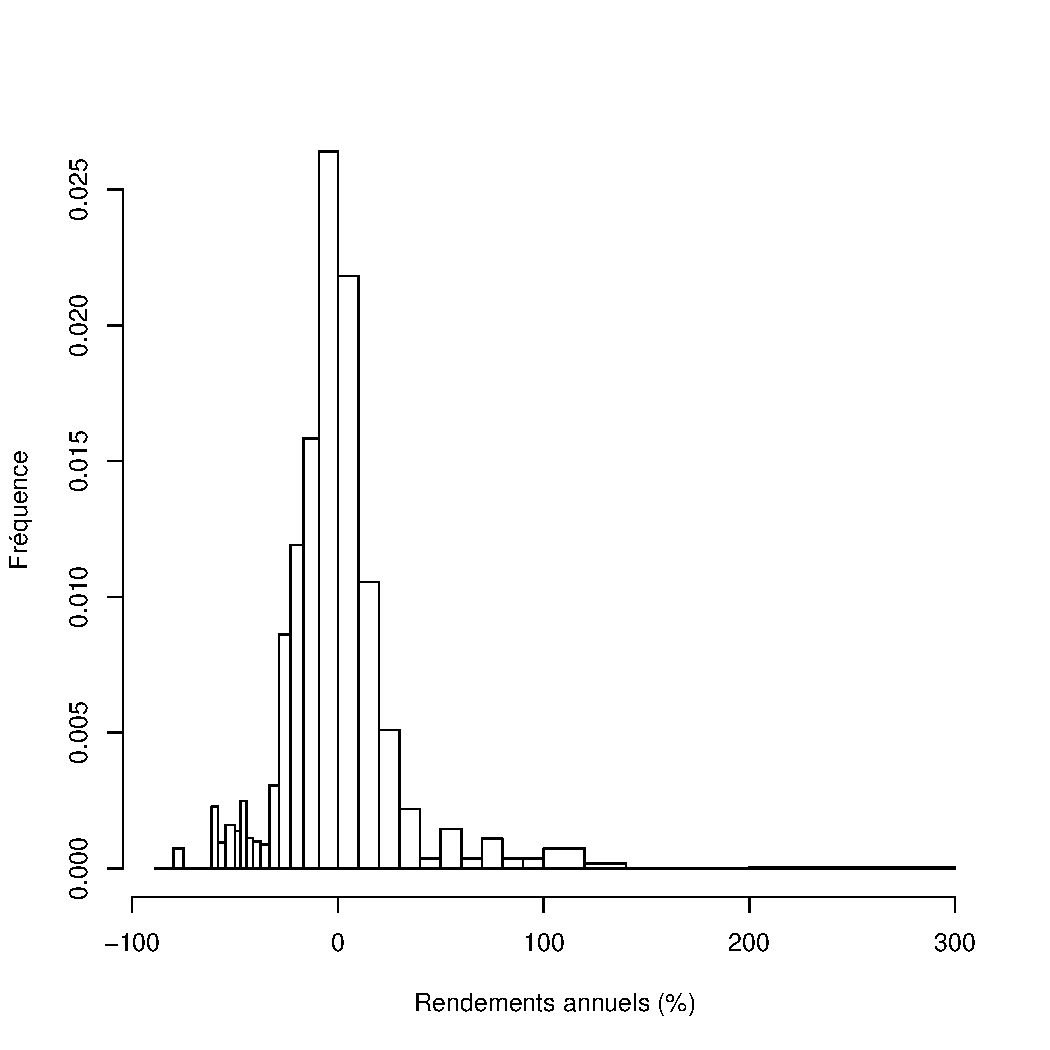
\includegraphics[scale=0.75]{../graphiques/mitchell1.pdf}
  \caption{Distribution des rendements annuels de 40 titres boursiers,
    de 1890 à 1915, Table XVIII de \cite{mitchell1916critique}}
  \label{fig:mitchell1}
\end{figure}

De plus, les variations extrêmes sont plus fréquentes que ne pourrait
le prédire un modèle basé sur un mouvement brownien. La distribution
des rendements aurait donc des queues plus épaisses
\footnote{traduction de l'anglais heavy tailed} que la normale. On
doit trouver un modèle qui permet de tenir compte de ces
particularités.

\subsection{Proposition de Mandelbrot}
\label{sec:mandelbrot}


\cite{mandelbrot1963variation} propose un modèle qui vise à combler
les lacunes du processus brownien géométrique
\eqref{eq:browniengeom}. Il explique que les distributions empiriques
des changements de prix sont habituellement trop \emph{pointues} pour
être considérées comme des échantillons d'une population gaussienne.

Il identifie différentes caractéristiques qu'un bon modèle des
rendements financiers devrait posséder:

\begin{enumerate}
  \label{enum:mandelbrot}
\item Il doit tenir compte de la fréquence des grands changements de
  prix. Il doit donc être basé sur une distribution leptocurtique,
  plus pointue au centre que la normale.
\item Il doit permettre des changements instantanés et imprévisibles
  de toute amplitude.
\item Il doit admettre une probabilité non nulle que plusieurs
  changements consécutifs semblent corrélés.
\item Il doit admettre un processus de prix non stationnaire, car la
  variance échantillonnale prend différentes valeurs à travers le
  temps.
\end{enumerate}

La famille de distributions L stable semble être celle qui répond le
mieux à l'ensemble de ces conditions \citep{walterlevy}. L'équation
suivante définit la propriété de L-stabilité de la distribution de la
variable aléatoire des rendements sur une période $R$:
\begin{align}
  (a_1 R_1 + b_1) + (a_2 R_2 + b_2) &\stackrel{d}{=} aR + b \\
  \forall a_1,a_2 > 0, \forall b_1, b_2.
\end{align}

La solution générale de cette équation a été découverte par Lévy en
1925. Le logarithme de la fonction caractéristique de celle-ci prend
la forme suivante:
\begin{align}
  \ln{(\phi_{R}(\xi))} = i\delta \xi - \gamma |\xi|^{\alpha}
  \left[1+\frac{i\beta \xi}{|\xi|} \tan{\frac{\alpha\pi}{2}} \right].
\end{align}

Le domaine et le rôle des paramètres de la distribution L stable est
décrit à la table \ref{tab:roleparam}. La flexibilité apportée par les
quatre paramètres permet de remplir les quatre conditions établies au
début de cette section. De plus, l'absence, dans la majorité des cas,
de moments finis d'ordre supérieur à l'espérance, permet de tenir
compte du mouvement erratique des prix et ainsi produire de larges
discontinuités de son processus. Elle permet aussi d'expliquer
l'apparence de corrélation sérielle, en considérant une probabilité
non négligeable que cette caractéristique soit présente. Cependant, ce
modèle est difficile à appliquer à l'évaluation de produits dérivés
pour cette raison, étant donné que l'on devra être en mesure de
quantifier la volatilité.
\begin{table}[!ht]
  \centering
  \begin{tabular}{|c|p{1.75cm}|p{2.5cm}|p{6.25cm}|}
    \hline
    \textbf{Paramètre} & \textbf{Domaine} & \textbf{Rôle} & \textbf{Observations} \\
    \hline
    $\alpha$ & $\left]0,2\right]$ & Aplatissement & Plus sa valeur est petite, plus la distribution est leptocurtique. $\alpha=2$ correspond à la distribution normale. \\
    $\beta$ & $\left] -1, 1 \right]$ & Asymétrie & Défini seulement lorsque $\alpha \neq 1$. Lorsque $\alpha=1$ et $\beta=0$, on obtient la distribution de Cauchy.  \\
    $\gamma = s^{\alpha}$ & $\mathbb{R}\setminus\{0 \}$ & Échelle & On doit prendre la racine $\alpha$ pour obtenir un paramètre d'échelle $s$ tel que défini par Pearson. \\
    $\delta$ & $\mathbb{R}$ & Localisation & \\
    \hline
  \end{tabular}
  \caption{Domaine et rôle des paramètres de la distribution L stable de Mandelbrot}
  \label{tab:roleparam}
\end{table}

L'approche classique, selon Mandelbrot, pour expliquer les grands
changements de prix a été de considérer un mélange de deux
distributions normales, dont une pour les fluctuations régulières et
une qui a une variance plus importante, pour les discontinuités. Il
remarque que pour expliquer adéquatement le comportement des données
empiriques, on doit introduire un mélange de plusieurs distributions
normales, ce qui rendrait le modèle plus complexe. Par contre, on
retrouve une approche intéressante avec le modèle présenté à la
section suivante.

\subsection{Le modèle de Press}
\label{sec:press}

\cite{press1967compound} propose un modèle statistique basé sur un
processus de Poisson composé auquel on ajoute un mouvement brownien
$W(t)$. C'est donc d'un processus ayant des incréments stationnaires
et indépendants. Il présente donc les caractéristiques d'un processus
de Lévy. Press utilise aussi la transformation logarithmique
\eqref{eq:browniengeom} afin que la variation soit proportionnelle au
prix. Il remarque aussi que le modèle logarithmique de Bachelier est
inadéquat, car il ne tient pas compte des queues de la distribution
empirique des rendements qui sont plus épaisses que celles de la
normale. Il ajoute que le modèle proposé par Mandelbrot est
discutable, car il ne trouve aucune évidence, à partir des données
observées, que la distribution de la population aurait une variance
infinie.

Le processus de Poisson $\left\{N(t)\right\}$ de paramètre $\lambda t$
est un processus de comptage qui détermine les occurrences des sauts
$Y_k, k = 1, \ldots, N(t)$. Ces sauts surviennent généralement
lorsqu'une information importante est rendue publique par rapport à un
titre. Ceux-ci sont aussi de distribution normale, mais leur espérance
n'est pas nulle et leur variance est différente de celle du processus
$W(t)$. Cette composante que l'on ajoute au modèle de Bachelier
modifié permet d'expliquer les variations plus importantes et moins
fréquentes observées empiriquement.

Le processus du logarithme du prix $\left\{s(t)\right\} \equiv
\left\{\ln{(S(t))}\right\}$ est donc représenté par l'équation
suivante:
\begin{align}
  \label{eq:press67}
  s(t) &= s(0) + \sum_{k=1}^{N(t)} Y_k + W(t).
\end{align}

On définit les différentes variables aléatoires composant le processus
comme suit:
\begin{align*}
  Y_k &\sim N(\theta,\sigma_2^2) \\
  W(t) &\sim N(0,\sigma_1^2 t) \\
  N(t) &\sim Poisson(\lambda t)
\end{align*}

Comme pour la plupart des processus de Lévy, on ne peut obtenir une
forme explicite pour la fonction de densité, car celle-ci se présente
sous la forme d'une série infinie. On représente alors ces processus
par leur fonction caractéristique, formée par le produit de celles de
leurs différentes composantes.

La distribution du logarithme du prix $s(t)$ est définie par la
fonction caractéristique $\phi_{s(t)}(\xi)$, qui est le produit de
celle de la constante et celles des processus de Wiener et de Poisson
composé:
\begin{align}
  \label{eq:fncaractpress}
  \phi_{s(t)}\left(\xi\right) &= E\left[e^{i \xi s(t)} \right] \nonumber \\
  &= exp\left\{ i\xi \cdot s(0) \right\} \times exp \left\{ -\frac{t \sigma_1^2 \xi^2}{2} \right\} \times exp \left\{ \lambda t \left[e^{i \theta \xi-(\sigma_2^2 \xi^2/2)}-1 \right] \right\} \nonumber \\
  &= exp\left\{ i\xi \cdot s(0)- \frac{t}{2}\sigma_1^2\xi^2 + \lambda
    t \left[e^{i \theta \xi-(\sigma_2^2 \xi^2/2)}-1 \right] \right\}.
\end{align}

Afin d'estimer le modèle, on s'intéressera plutôt à la distribution
d'un incrément $\Delta s(t) = s(t)-s(t-1)$ de ce processus. La
fonction caractéristique $\phi_{\Delta s(t)}(\xi)$ de cette variable
aléatoire peut être facilement identifiée à partir de celle du
processus \eqref{eq:fncaractpress}. Essentiellement, on pose $s(0)=0
\mbox{ et } t=1$, pour obtenir:
\begin{align}
  \label{eq:fncaractpress2}
  \phi_{\Delta s(t)}\left(\xi\right) &= E\left[e^{i\xi\Delta s(t)} \right] \nonumber \\
  &= exp\left\{-\frac{\sigma_1^2 \xi^2}{2} + \lambda \left[e^{i
        \xi\theta -(\sigma_2^2 \xi^2/2)}-1 \right] \right\}.
\end{align}

Pour estimer les paramètres du modèle, on privilégie la méthode des
cumulants, qui est similaire à la méthode des moments. Considérons les
quatre premiers cumulants de la distribution de l'incrément $\Delta
s(t)$:
\begin{subequations}\label{eq:cumulantspress}
  \begin{align}
    K_1 &= \lambda\theta \\
    K_2 &= \sigma_1^2+\lambda(\theta^2+\sigma_2^2) \\
    K_3 &= \lambda\theta(\theta^2+3\sigma_2^2) \\
    K_4 &= \lambda(\theta^4 + 6 \theta^2 \sigma_2^2 + 3 \sigma_2^4).
  \end{align}
\end{subequations}

En utilisant les quatre premiers cumulants empiriques
\eqref{eq:cumulantsempiriques}, on obtient les équations suivantes:
\begin{subequations}\label{eq:presscum}
  \begin{align}
    0 &= \hat\theta^4 - \frac{\overline{K}_3}{\overline{K}_1} \hat\theta^2 + \frac{3\overline{K}_4}{2\overline{K}_1} \hat\theta - \frac{\overline{K}_3^2}{2\overline{K}_1^2} \label{eq:presscumtheta}\\
    \hat\lambda &= \frac{\overline{K}_1}{\hat\theta} \label{eq:presscumlambda}\\
    \hat\sigma_2^2 &= \frac{\overline{K}_3-\hat\theta^2\overline{K}_1}{3\overline{K}_1} \label{eq:presscumsigma2}\\
    \hat\sigma_1^2 &= \overline{K}_2 -
    \frac{\overline{K}_1}{\hat\theta}\left(\hat\theta^2 +
      \frac{\overline{K}_3 - \overline{K}_3 \theta^2}{3\overline{K}_1}
    \right). \label{eq:presscumsigma1}
  \end{align}
\end{subequations}

En résolvant numériquement l'équation \eqref{eq:presscumtheta} pour le
$\hat\theta$, puis par substitutions successives dans les équations
\eqref{eq:presscum}, on obtient des estimateurs convergents pour les
quatre paramètres du modèle.

Un modèle similaire a aussi été présenté par \cite{merton1976option},
cependant, il inclut un paramètre de dérive $\alpha$, et considère que
les sauts $Y$, qui sont des facteurs multiplicatifs, peuvent suivre une autre distribution que la normale. Il
présente le modèle sous la forme d'une équation différentielle
stochastique:
\begin{align}
  \label{eq:modelemerton}
  \frac{dS}{S} = (\alpha - \lambda k)dt + \sigma dW + dq.
\end{align}
La constante $k$ représente l'espérance de la variation relative si un
saut se produit et $q$, le processus de Poisson composé. La solution
de cette équation est, selon le lemme d'Itô:
\begin{align}
  S(t) &= \tilde{S}(0) \exp \left\{
    (\alpha-\frac{1}{2}\sigma^2-\lambda k)t +
    \sigma W(t) \right\}
    \end{align}
    où
    \begin{align}
  \tilde{S}(0) &= \begin{cases}
    S(0) & \text{si } N(t) = 0\\
    S(0) \sum_{k=1}^{N(t)} Y_k & \text{si } N(t) \geq 1. \nonumber
  \end{cases}
\end{align}

En spécifiant un paramètre de dérive $\delta =
\alpha-\frac{1}{2}\sigma^2-\lambda k$ et en considérant que les
sauts $Y$ sont de distribution lognormale, on peut réécrire la
fonction caractéristique d'un incrément \eqref{eq:fncaractpress2} du
modèle de Press:
\begin{align}
  \label{eq:fncaractmerton}
  \phi_{\Delta s(t)}\left(\xi\right) &= E\left[e^{i\xi\Delta s(t)} \right] \nonumber \\
  &= \exp\left\{i\delta \xi -\frac{\sigma^2 \xi^2}{2} + \lambda
    \left[e^{i \xi\theta -(\sigma^2 \xi^2/2)}-1 \right] \right\}.
\end{align}

L'utilisation de ce modèle présente deux désavantages. L'estimation du
modèle est difficile lorsque la moyenne s'approche de 0, car le
quotient \eqref{eq:presscumlambda} tend alors vers une
indétermination. De plus, contrairement à d'autres modèles, il est
difficile d'identifier le rôle des paramètres par rapport à un moment
en particulier (classification de Pearson), contrairement à ce qu'on
pourra observer avec la distribution de Laplace asymétrique
généralisée.

\subsection{Le modèle de Praetz}

\cite{praetz1972distribution} propose un modèle inspiré par la
physique des particules. Il pose comme hypothèse que deux intervalles
qui ne se chevauchent pas forment une marche aléatoire, et que les
éléments qui composent la séquence des rendements financiers $\left\{
  R(t) \right\}$ sont mutuellement indépendants. Il considère qu'un
état stable existe où les rendements suivent une loi normale de
paramètres $\mu$ et $\sigma^2$.

Cependant, cet état stable n'est jamais réellement atteint, et la
fonction de densité empirique généralement observée suppose une
distribution symétrique concave, pointue au centre et ayant des queues
épaisses. Il fait une analogie entre la température d'un gaz et le
niveau d'activité sur les marchés, où la variance du mouvement
brownien est proportionnelle à ces deux quantités. Il propose que le
paramètre de variance de la normale $\sigma^2$ suive une distribution
$g(\sigma^2)$ ayant un support positif. La distribution conditionnelle
est normale lorsque ce paramètre est connu.
\begin{align}
  h_{R(t)}(r) &= \int_0^{\infty} f_{R(t)}(r|\sigma^2) g(\sigma^2) d\sigma^2 \\
  f_{R(t)}(r|\sigma^2) &= \frac{1}{\sigma\sqrt{2\pi}}exp\left\{-\frac{(r-\mu)^2}{2\sigma^2} \right\} \label{eq:praetz72}
\end{align}

Il propose comme solution acceptable pour la densité $g(\sigma^2)$, la
distribution gamma inverse de paramètres $m$ et $s^2$:
\begin{align}
  \label{eq:gpraetz}
  g(\sigma^2) &=
  \frac{s^{2m}(m-1)^me^{-(m-1)\frac{s^2}{\sigma^2}}}{\sigma^{2(m-1)}\Gamma(m)}.
\end{align}

Cette distribution a pour moyenne $s^2$ et variance $\frac{s^2}{m-2}$.
La distribution non conditionnelle des rendements $h_{R(t)}$ est
approximativement une Student avec $2m$ degrés de liberté à un facteur
d'échelle de $\left(\frac{m}{m-1}\right)^{1/2}$ près:
\begin{align}
  \label{eq:hpraetz}
  h_{R(t)}(r) &= \frac{\Gamma(m)\left[\ 2(m-1)\pi
    \right]^{1/2}s}{\left[1+\frac{(y-\mu)^2}{s^2(2m-2)}
    \right]^{m+1/2}}.
\end{align}

D'autres distributions pourraient être utilisées au lieu de la gamma
inverse. En utilisant la loi gamma, on obtient la distribution de
Laplace asymétrique généralisée, qui sera l'objet d'une étude
approfondie aux chapitres suivants. Il propose enfin d'utiliser aussi
la distribution a priori gamma inverse pour le paramètre $\mu$. Par
contre, il remarque qu'il obtient aussi une distribution similaire à
celle de Student. Cette généralisation n'est donc pas nécessaire.

\section{Conditions essentielles de Madan et Seneta}
\label{sec:madanseneta90}

Inspirés par les travaux de Mandelbrot, Press et Praetz,
\cite{madan1990variance} présentent un ensemble de conditions
considérées essentielles dans l'élaboration d'un modèle de rendements
financiers. Ils se baseront sur celles-ci pour proposer le modèle
Variance Gamma:

\begin{enumerate}
\item La distribution des rendements $R$ doit avoir une queue
  épaisse. Ainsi, la probabilité que cette variable aléatoire ait une
  valeur supérieure à $r+t$ avec un $t$ petit, sachant qu'elle est
  supérieure à $r$, doit tendre vers 1, ce qui signifie que la
  fonction de survie converge lorsque cette quantité est grande.
  \begin{eqnarray}
    \label{eq:condmadan1}
    \lim_{r\rightarrow \infty} P\left[R > r+t | R > r \right] &=& 1 \\
    \bar{F}(r+t) &\sim& \bar{F}(r), \qquad r \rightarrow \infty \nonumber
  \end{eqnarray}
\item La distribution doit posséder des moments finis pour les $n$
  premières puissances des rendements $R$. Étant donné que l'on
  cherche à modéliser la queue de la distribution, on fixe $n=4$.
  \begin{equation}
    \label{eq:condmadan2}
    E\left[R^k\right] < \infty, \qquad k \in \lbrace 1,2,3,4 \rbrace
  \end{equation}
\item
  \begin{enumerate}
  \item Le modèle doit proposer un processus de temps continu ayant
    des accroissements stationnaires et indépendants.
  \item Les distributions des accroissements doivent appartenir à la
    même famille, quelle que soit leur longueur. Cette condition est
    essentielle afin de permettre l'échantillonnage et l'analyse des
    séries chronologiques.
  \end{enumerate}
\item Le modèle doit permettre une extension multivariée avec une
  distribution elliptique afin de conserver la validité du modèle
  d'évaluation des actifs financiers.
\end{enumerate}

Chacun des modèles présentés précédemment respecte la majorité ou
toutes ces conditions. Les résultats se retrouvent à la table
\ref{tab:condmadan}.
\begin{table}[!ht]
  \centering
  \begin{tabular}{ccccc}
    & \multicolumn{4}{c}{\textbf{Conditions}} \\
    \hline
    \textbf{Modèles}                                       & 1 & 2 & 3 & 4 \\
    \hline
    Mouvement brownien de Bachelier              &   & $\ast$ & $\ast$ & $\ast$ \\
    Distribution stable symétrique de Mandelbrot & $\ast$ & & & $\ast$ \\
    Processus de Poisson composé de Press       & $\ast$ & $\ast$ & $\ast$ & $\ast$ \\
    Mélange gaussien/inverse gamma de Praetz     & $\ast$ & $\ast$ &   & $\ast$ \\
    Modèle Variance Gamma de Madan et Seneta     & $\ast$ & $\ast$ & $\ast$ & $\ast$ \\
    \hline
  \end{tabular}
  \caption{Respect des conditions émises par Madan et Seneta pour les différents modèles présentés}
  \label{tab:condmadan}
\end{table}

On remarque que le modèle de Press remplit toutes les conditions
émises par Madan et Seneta. Cependant, ils remarqueront que ce n'est
pas un processus de sauts, car il contient aussi une composante de
diffusion (Section \ref{sec:levykhintchine}), ce qui va à l'encontre
de l'intuition derrière la continuité de la trajectoire du prix. C'est
cette dernière observation qui les incitera à proposer le modèle
Variance Gamma, qui est un processus de sauts. Ce modèle, aussi étudié
sous le nom de distribution de Laplace asymétrique généralisée par
\cite{kotz2001laplace}, a acquis beaucoup de notoriété dans le domaine
de la finance mathématique. De plus, avec le développement de
l'informatique et des méthodes numériques, on peut maintenant utiliser
de manière efficace la fonction caractéristique dans le cadre de la
calibration, des tests statistiques et de la tarification
d'options. C'est pourquoi un intérêt particulier est apporté à cette
distribution dans ce texte.

% \section{La volatilité}
% \label{sec:volatilite}

% La \textbf{volatilité} est une mesure de l'ampleur des variations du
% prix d'un actif. Elle sert à quantifier le risque lié à un
% investissement, le plus souvent sur un horizon à court terme. Elle se
% calcule le plus souvent à partir des prix des options observés sur les
% marchés, on parle alors de volatilité implicite. Comme elle n'est pas
% mesurable, cette volatilité est le reflet de l'anticipation des
% investisseurs quant aux perspectives du marché.

% Cependant, on peut toujours mesurer la volatilité historique du prix
% d'un titre à travers les rendements passés. La première étude à ce
% sujet a été faite par Black et Scholes, les auteurs du célèbre modèle
% qui porte désormais leur nom. Ils ont conclu que leur modèle
% surestimait le prix des options pour des actifs sous-jacents ayant une
% volatilité historique élevée, le contraire se produisait lorsqu'elle
% l'était peu. Leur modèle est donc utile à condition que les
% investisseurs puissent faire de bonnes prévisions
% \citep{musiela2005martingale}.

% De plus, comme il a été expliqué précédemment, les données historiques
% démontrent que la volatilité n'est pas constante avec le temps, mais
% plutôt aléatoire. Dans cette perspective, on pourrait identifier la
% distribution de la volatilité à travers le temps.
% \subsection{Mesure de la volatilité historique}
% \label{sec:mesurevolatilite}

% Afin d'obtenir un ensemble d'observations de la volatilité historique,
% on utilise une approche par fenêtre mobile. \cite{randal2004non}
% considère un estimateur de variance mobile $\hat\sigma^2(t)$, basé sur
% les rendements centrés $R(t) = Y(t)-E\left[Y(t)\right]$ de la forme
% \begin{align}
%   \hat\sigma^2(t) = \frac{1}{2r+1} \sum_{j=-r}^r R(t+j)^2, \qquad
%   t\in\left[r+1,n-r\right] \label{mobilevariance}
% \end{align}

% Étant donné la taille limitée $n$ de l'échantillon des rendements, on
% doit faire un compromis entre la précision des observations de la
% volatilité et le nombre $n-2r$ de celles-ci. L'hypothèse de volatilité
% stochastique fera pencher en faveur d'une fenêtre étroite, ce qui
% procurera un grand nombre d'observations la décrivant à court
% terme. On pourra donc ajuster une distribution de probabilités à
% celles-ci.

% \subsection{Biais de la volatilité implicite}
% \label{sec:impvolsmile}

% Le biais de volatilité implicite est un concept qui explique pourquoi
% la volatilité des options croît lorsque le prix d'exercice s'éloigne
% de la valeur actuelle du titre sous-jacent. Selon
% \cite{hull1999options}, ce phénomène a été remarqué sur les marchés
% financiers américains à partir du krach boursier du lundi noir
% \footnote{19 octobre 1987}, et n'est toujours pas entièrement
% expliqué. Généralement, on observe que, pour les options sur indices
% boursiers et taux de change, la courbe de volatilité implicite est
% plutôt symétrique, alors qu'elle est asymétrique pour celles sur
% actions (voir figure \ref{fig:volimplicite} pour un exemple).
% \begin{figure}[!ht]
%   \centering
%   \includegraphics[]{./bbry-echeance-06-2013-20mai2013.png}
%   \caption{Courbe de volatilité implicite, titre BBRY, option d'achat
%     avec échéance 06-2013, observée le 20-05-2013, prix de 15.83,
%     source: \cite{thevolskew}}
%   \label{fig:volimplicite}
% \end{figure}

%%% Local Variables: 
%%% mode: latex
%%% TeX-master: "gabarit-maitrise"
%%% End: 
             % chapitre 1
\chapter{La distribution de Laplace asymétrique
  généralisée} % numéroté

Dans ce chapitre, on présente, en premier lieu, le processus de
Laplace ainsi que les deux processus sous-jacents à sa construction,
le processus gamma et le processus de Wiener. Ensuite, on présente la
distribution de Laplace asymétrique généralisée et ses principales
propriétés qui seront utilisées pour modéliser les rendements de
titres financiers. Puis, on présente quelques cas particuliers.  Dans
le chapitre suivant, on présentera différentes méthodes pour obtenir
une approximation de la fonction de densité et la fonction de
répartition.

La distribution de Laplace asymétrique généralisée a été
principalement étudiée par \cite{kozubowski1999class}. Cependant, elle
a été introduite près d'une décennie auparavant par
\cite{madan1990variance}, sous le nom de distribution Variance
Gamma. La différence entre les approches des deux auteurs est
majeure. \cite{madan1990variance} développent un modèle financier à
partir du mouvement brownien géométrique, qu'ils généralisent en
proposant que la variance suive une distribution
gamma. \cite{kozubowski1999class} généralisent la distribution de
Laplace asymétrique. Leur approche est plus générale, car ils ne
cherchent pas à développer un modèle financier, mais une nouvelle
classe de distributions utilisable dans divers domaines
scientifiques. Étant donné leur approche plus détaillée et plus
intuitive, c'est leur formulation du modèle qui sera développée. On
rappellera enfin que les deux modèles sont équivalents même si leurs
paramétrisations sont différentes.

\section{Le processus de Laplace}
\label{sec:processusGAL}

Le processus de Laplace est défini comme étant un processus de Wiener
subordonné par un processus gamma. En d'autres termes, c'est un
processus de Wiener évalué à des temps aléatoires déterminés par un
processus gamma. Selon \cite{kotz2001laplace}, ce dernier est à la
distribution de Laplace ce que le mouvement brownien est à la loi
normale. Il est aussi un cas particulier des processus de Lévy, et en
conserve donc la principale propriété, celle d'être infiniment
divisible.

Il a certains points en commun avec le mouvement brownien dont des
moments finis pour tout ordre et des incréments indépendants et
stationnaires. Cependant, la plupart des caractéristiques diffèrent:
\begin{itemize}
\item Discontinuité des trajectoires (processus de sauts);
\item Distribution asymétrique des accroissements;
\item Paramètres d'échelle et de temps entièrement dissociés.
\end{itemize}

Enfin, il possède une représentation alternative qui n'implique aucun
processus de Wiener. Il peut en fait être représenté comme la
différence de deux processus gamma indépendants. On peut le
représenter en utilisant la forme générale des processus de Lévy.

\subsection{Le processus gamma}
\label{sec:processusgamma}

Le processus gamma, noté $\left\{G(t;\tau,\beta)\right\}$, est un
processus de sauts purs (donc aucune composante de dérive ni de
diffusion) dont les incréments $G(t+1;\tau,\beta) - G(t;\tau,\beta)$
suivent une distribution gamma de paramètres de forme $\tau$ et
d'échelle $\beta$, définie par les fonctions de densité
$f_{\tau,\beta}(x)$ et caractéristique $\phi_{\tau,\beta}(\xi)$:
\begin{align}
  f_{\tau,\beta}(x) &= \frac{\beta^\tau}{\Gamma(\tau)} x^{\tau \,-\, 1} e^{- \beta x } 1_{\lbrace x\geq\,0 \rbrace} \label{eq:densitegamma} \\
  \phi_{\tau,\beta}(\xi) &= E\left[e^{i\xi\,X} \right] \nonumber\\
  &= \int_{0}^{\infty} e^{i\xi\,x} f_{\tau,\beta}(x) dx \nonumber\\
  &=
  \frac{1}{\left(1-\frac{i\xi}{\beta}\right)^{\tau}} \label{eq:fncaractgamma}.
\end{align}

On s'intéresse à la situation où le paramètre d'échelle est de valeur
unitaire ($\beta=1$). Le processus gamma agit alors à titre de
compteur et sa valeur $G(t;\tau,\beta=1)$ au temps $t$ correspondra au
nombre de sauts depuis $t=0$. La fonction de densité
$G(t+1;\tau,\beta=1) - G(t;\tau,\beta=1)$ sera alors:
\begin{align}
  f_{\tau,\beta=1}(x) &= \frac{1}{\Gamma(\tau)} x^{\tau \,-\, 1} e^{- x} 1_{\lbrace x\geq\,0 \rbrace}. \label{eq:densitegamma1}
\end{align}

Le paramètre $\tau$, qui définit la forme de la distribution,
déterminera la fréquence moyenne des sauts du processus gamma
$\Gamma(t;\tau,\beta=1)$, étant donné l'espérance $E[G(t)] = \tau\cdot
t$. La fonction caractéristique de ce processus sera donc
$\phi(\xi,t;\tau,\beta=1)$, en utilisant la propriété de convolution
\eqref{eq:convocaractIID} (même si le temps $t$ n'est pas entier, car
la distribution est infiniment divisible):
\begin{align}
  \phi(\xi,t;\tau,\beta=1) &= \left[\frac{1}{\left(1-\frac{i\xi}{1}\right)^{\tau}}\right]^t \nonumber\\
  &= \frac{1}{\left(1-i\xi\right)^{\tau\cdot t}}.
\end{align}

On peut réécrire la fonction caractéristique d'un incrément de ce
processus $\phi(\xi;t=1;\tau,\beta=1)$ sous la représentation de
Lévy-Khintchine \eqref{eq:levykhintchine}, avec l'exposant
caractéristique $\Xi(\zeta)$:
\begin{align}
  \label{eq:exposantchargamma}
  \Xi(\zeta;t=1;\tau,\beta=1) &= \tau\ln{\left(1-i\zeta\right)} \\
  &= \tau \left(e^{0} - e^{-\infty}\right) \ln{\left(1-i\zeta \right)} \nonumber\\
  &= \tau \int_{0}^{\infty} \frac{e^{-x} - e^{-(1-i\zeta)x}}{x} dx \nonumber\\
  &\qquad\mbox{(intégrale de Frullani \citep{spiegel1999schaum}, p.115)} \nonumber\\
  &= \tau \int_{0}^{\infty}
  \left(1-e^{i\zeta\,x}\right)\frac{1}{x}e^{-x}dx.
\end{align}

On a donc, par cette représentation, la démonstration que le processus
gamma est un processus de sauts purs. Il pourra donc être utilisé
comme subordonnant dans la construction d'un processus subordonné
\eqref{eq:processussubordonne}.

\subsection{Le processus de Wiener}
\label{sec:mouvementbrownien}

Le processus de Wiener $\left\{W(t;\mu,\sigma^2)\right\}$ est un
processus de diffusion avec dérive. Il n'a donc pas de composante de
saut. Ses incréments suivent une distribution normale:
\begin{align}
  \label{eq:incrwiener}
  W(t+1;\mu,\sigma^2) - W(t;\mu,\sigma^2) \sim N(\mu,\sigma^2).
\end{align}
Cette distribution est définie par la fonction de densité
$f_{\mu,\sigma}(x)$ et la fonction caractéristique
$\phi_{\mu,\sigma}(\xi)$:
\begin{align}
  f_{\mu,\sigma}(x) &= \frac{1}{\sqrt{2\pi\sigma^2}}\exp{-\left\{\frac{1}{2} \left(\frac{x-\mu}{\sigma} \right)^2\right\}} \label{eq:fndensitenormale} \\
  \phi_{\mu,\sigma}(\xi) &= \exp\left\{
    i\mu\xi-\frac{\sigma^2\xi^2}{2}
  \right\} \label{eq:fncaractnormale}.
\end{align}

Notons que la variance d'un incrément est proportionnelle à la
longueur de celui-ci.  Soit deux incréments indépendants d'un même
processus: $I_1 = W(t+q;\mu,\sigma^2) - W(t;\mu,\sigma^2) \sim
N(q\mu,q\sigma^2) \mbox{ et } I_2 = W(t+q+s;\mu,\sigma^2) -
W(t+q;\mu,\sigma^2) \sim N(s\mu,s\sigma^2)$. La somme de ces
incréments suit une distribution normale dont la moyenne et la
variance sont respectivement la somme de celles des deux incréments:
\begin{align}
  I_1+I_2 \sim N((q+s)\mu, (q+s)\sigma^2).
\end{align}

Comme la distribution normale est aussi infiniment divisible, on peut
obtenir la fonction caractéristique du processus
$\phi(\xi;t;\mu,\sigma^2)$ en utilisant la propriété de convolution
\eqref{eq:convocaractIID}:
\begin{align}
  \phi(\xi;t;\mu,\sigma^2) = \exp\left\{ i\mu t
    \xi-\frac{\sigma^2t\xi^2}{2} \right\}.
\end{align}

On déduit donc facilement l'exposant caractéristique
$\Lambda(\xi;t=1;\mu,\sigma^2)$ d'un incrément de ce processus, sous
la représentation de Lévy-Khintchine:
\begin{align}
  \label{eq:exposantcaractnormale}
  \Lambda(\xi;t=1;\mu,\sigma^2) = -(i\mu \xi-\frac{\sigma^2\xi^2}{2}).
\end{align}

Ceci démontre que le processus de Wiener est un processus avec dérive
et diffusion, mais sans composante de saut. Il pourra donc être
utilisé pour construire un processus subordonné
\eqref{eq:processussubordonne}.

\subsection{Le processus de Laplace est un processus subordonné}
\label{sec:browniensub}

On considère un processus gamma $G(t;\tau,\beta=1)$ et un processus de
Wiener $W(t;\mu,\sigma^2)$. On se rappelle que la variance d'un
incrément \eqref{eq:incrwiener} de ce dernier est proportionnelle à la
longueur de l'intervalle de temps. En utilisant une propriété appelée
la subordination, on peut modifier l'échelle de temps du processus de
Wiener de sorte que la variance soit aléatoire pour tout intervalle
. Tout processus de Lévy peut être utilisé comme subordonnant pour
définir cette échelle de temps. Si on utilise le processus gamma, on
obtiendra le processus de Laplace sans dérive
$\left\{Y(t;\sigma,\mu,\tau)\right\}$ défini comme suit:
\begin{align}
  \label{eq:VGsubordinne}
  \lbrace Y(t;\sigma,\mu,\tau)\rbrace &\equiv \lbrace
  W(G(t;\tau,\beta=1);\mu,\sigma^2)\rbrace.
\end{align}

On obtient l'exposant caractéristique $\Psi(\xi,t=1;\sigma,\mu,\tau)$
d'un incrément $Y(t+1;\sigma,\mu,\tau)-Y(t;\sigma,\mu,\tau)$ en
utilisant la propriété de subordination définie par l'équation
\eqref{eq:exposantcaractYt}, où $\Xi(\zeta,t=1;\tau,\beta=1)$ est
l'exposant caractéristique du processus gamma et
$\Lambda(\xi,t=1;\mu,\sigma^2)$ celui du processus de Wiener:
\begin{align}
  \label{eq:exposantcaractLaplace}
  \Psi(\xi,t=1;\sigma,\mu,\tau) &= \Xi(i\Lambda(\xi,t=1;\mu,\sigma^2),t=1;\tau,\beta=1) \nonumber\\
  &= \tau \ln{\left(1-i(i\Lambda(\xi)) \right)} \nonumber\\
  &= \tau \ln{\left(1+(\frac{\sigma^2 \xi^2}{2} - i \mu \xi) \right)}.
\end{align}

Le processus de Laplace sans dérive est donc, par définition, un
processus de Lévy et par conséquent infiniment divisible. En utilisant
l'exposant caractéristique \eqref{eq:exposantcaractLaplace} et la
définition \eqref{eq:fncaractYt}, on obtient sa fonction
caractéristique:
\begin{align}
  \label{eq:fonctioncaractlaplacesansdrift}
  \phi_{Y(t;\sigma,\mu,\tau)}(\xi) &= \exp{\left\{-t \cdot \Psi(\xi,t=1;\sigma,\mu,\tau)\right\}} \nonumber\\
  &= \exp{\left\{-t \cdot \left(\tau \ln{\left(1+(\frac{\sigma^2
              \xi^2}{2} - i \mu
            \xi) \right)} \right)\right\}} \nonumber\\
  &= \left(1+\frac{\sigma^2 \xi^2}{2} - i \mu \xi\right)^{-\tau \cdot
    t}.
\end{align}

Une manière simple pour expliquer le mécanisme derrière le processus
subordonné est d'en construire une trajectoire à l'aide de la
simulation.

On simule un temps d'arrivée $T_1$, de distribution gamma, puis une
hauteur de saut $X_1$, de distribution normale. On obtient ainsi le
premier incrément de la trajectoire, tel qu'illustré à la figure
\ref{fig:increment1}.
\begin{figure}[!ht]
  \centering % Graphic for TeX using PGF
% Title: /home/francois/projet-de-maitrise/graphiques/increment1.dia
% Creator: Dia v0.97.2
% CreationDate: Mon Jul 29 16:42:05 2013
% For: francois
% \usepackage{tikz}
% The following commands are not supported in PSTricks at present
% We define them conditionally, so when they are implemented,
% this pgf file will use them.
\ifx\du\undefined
  \newlength{\du}
\fi
\setlength{\du}{15\unitlength}
\begin{tikzpicture}
\pgftransformxscale{1.000000}
\pgftransformyscale{-1.000000}
\definecolor{dialinecolor}{rgb}{0.000000, 0.000000, 0.000000}
\pgfsetstrokecolor{dialinecolor}
\definecolor{dialinecolor}{rgb}{1.000000, 1.000000, 1.000000}
\pgfsetfillcolor{dialinecolor}
\pgfsetlinewidth{0.100000\du}
\pgfsetdash{}{0pt}
\pgfsetdash{}{0pt}
\pgfsetbuttcap
{
\definecolor{dialinecolor}{rgb}{0.000000, 0.000000, 0.000000}
\pgfsetfillcolor{dialinecolor}
% was here!!!
\pgfsetarrowsend{stealth}
\definecolor{dialinecolor}{rgb}{0.000000, 0.000000, 0.000000}
\pgfsetstrokecolor{dialinecolor}
\draw (19.200000\du,10.800000\du)--(28.800000\du,10.800000\du);
}
\pgfsetlinewidth{0.100000\du}
\pgfsetdash{}{0pt}
\pgfsetdash{}{0pt}
\pgfsetbuttcap
{
\definecolor{dialinecolor}{rgb}{0.000000, 0.000000, 0.000000}
\pgfsetfillcolor{dialinecolor}
% was here!!!
\pgfsetarrowsend{stealth}
\definecolor{dialinecolor}{rgb}{0.000000, 0.000000, 0.000000}
\pgfsetstrokecolor{dialinecolor}
\draw (19.200000\du,10.800000\du)--(19.200000\du,3.600000\du);
}
\pgfsetlinewidth{0.100000\du}
\pgfsetdash{}{0pt}
\pgfsetdash{}{0pt}
\pgfsetbuttcap
{
\definecolor{dialinecolor}{rgb}{0.000000, 0.000000, 0.000000}
\pgfsetfillcolor{dialinecolor}
% was here!!!
\definecolor{dialinecolor}{rgb}{0.000000, 0.000000, 0.000000}
\pgfsetstrokecolor{dialinecolor}
\draw (20.400000\du,10.600000\du)--(20.400000\du,11.000000\du);
}
\pgfsetlinewidth{0.100000\du}
\pgfsetdash{}{0pt}
\pgfsetdash{}{0pt}
\pgfsetbuttcap
{
\definecolor{dialinecolor}{rgb}{0.000000, 0.000000, 0.000000}
\pgfsetfillcolor{dialinecolor}
% was here!!!
\definecolor{dialinecolor}{rgb}{0.000000, 0.000000, 0.000000}
\pgfsetstrokecolor{dialinecolor}
\draw (26.400000\du,10.600000\du)--(26.400000\du,11.000000\du);
}
\pgfsetlinewidth{0.100000\du}
\pgfsetdash{}{0pt}
\pgfsetdash{}{0pt}
\pgfsetbuttcap
{
\definecolor{dialinecolor}{rgb}{0.000000, 0.000000, 0.000000}
\pgfsetfillcolor{dialinecolor}
% was here!!!
\definecolor{dialinecolor}{rgb}{0.000000, 0.000000, 0.000000}
\pgfsetstrokecolor{dialinecolor}
\draw (19.000000\du,9.600000\du)--(19.400000\du,9.600000\du);
}
% setfont left to latex
\definecolor{dialinecolor}{rgb}{0.000000, 0.000000, 0.000000}
\pgfsetstrokecolor{dialinecolor}
\node[anchor=west] at (20.200000\du,12.000000\du){0};
% setfont left to latex
\definecolor{dialinecolor}{rgb}{0.000000, 0.000000, 0.000000}
\pgfsetstrokecolor{dialinecolor}
\node[anchor=west] at (26.200000\du,12.000000\du){$T_1$};
% setfont left to latex
\definecolor{dialinecolor}{rgb}{0.000000, 0.000000, 0.000000}
\pgfsetstrokecolor{dialinecolor}
\node[anchor=west] at (18.200000\du,9.800000\du){0};
% setfont left to latex
\definecolor{dialinecolor}{rgb}{0.000000, 0.000000, 0.000000}
\pgfsetstrokecolor{dialinecolor}
\node[anchor=west] at (17.400000\du,6.200000\du){$X_1$};
\pgfsetlinewidth{0.100000\du}
\pgfsetdash{}{0pt}
\pgfsetdash{}{0pt}
\pgfsetbuttcap
{
\definecolor{dialinecolor}{rgb}{0.000000, 0.000000, 0.000000}
\pgfsetfillcolor{dialinecolor}
% was here!!!
\definecolor{dialinecolor}{rgb}{0.000000, 0.000000, 0.000000}
\pgfsetstrokecolor{dialinecolor}
\draw (19.000000\du,6.000000\du)--(19.400000\du,6.000000\du);
}
\pgfsetlinewidth{0.100000\du}
\pgfsetdash{}{0pt}
\pgfsetdash{}{0pt}
\pgfsetbuttcap
{
\definecolor{dialinecolor}{rgb}{0.000000, 0.000000, 0.000000}
\pgfsetfillcolor{dialinecolor}
% was here!!!
\definecolor{dialinecolor}{rgb}{0.000000, 0.000000, 0.000000}
\pgfsetstrokecolor{dialinecolor}
\draw (26.200000\du,6.000000\du)--(27.400000\du,6.000000\du);
}
\definecolor{dialinecolor}{rgb}{0.000000, 0.000000, 0.000000}
\pgfsetstrokecolor{dialinecolor}
\draw (26.200000\du,6.000000\du)--(27.400000\du,6.000000\du);
\pgfsetlinewidth{0.100000\du}
\pgfsetdash{}{0pt}
\pgfsetmiterjoin
\pgfsetbuttcap
\definecolor{dialinecolor}{rgb}{0.000000, 0.000000, 0.000000}
\pgfsetfillcolor{dialinecolor}
\pgfpathmoveto{\pgfpoint{26.200000\du}{6.000000\du}}
\pgfpathcurveto{\pgfpoint{26.200000\du}{5.875000\du}}{\pgfpoint{26.325000\du}{5.750000\du}}{\pgfpoint{26.450000\du}{5.750000\du}}
\pgfpathcurveto{\pgfpoint{26.575000\du}{5.750000\du}}{\pgfpoint{26.700000\du}{5.875000\du}}{\pgfpoint{26.700000\du}{6.000000\du}}
\pgfpathcurveto{\pgfpoint{26.700000\du}{6.125000\du}}{\pgfpoint{26.575000\du}{6.250000\du}}{\pgfpoint{26.450000\du}{6.250000\du}}
\pgfpathcurveto{\pgfpoint{26.325000\du}{6.250000\du}}{\pgfpoint{26.200000\du}{6.125000\du}}{\pgfpoint{26.200000\du}{6.000000\du}}
\pgfusepath{fill}
\definecolor{dialinecolor}{rgb}{0.000000, 0.000000, 0.000000}
\pgfsetstrokecolor{dialinecolor}
\pgfpathmoveto{\pgfpoint{26.200000\du}{6.000000\du}}
\pgfpathcurveto{\pgfpoint{26.200000\du}{5.875000\du}}{\pgfpoint{26.325000\du}{5.750000\du}}{\pgfpoint{26.450000\du}{5.750000\du}}
\pgfpathcurveto{\pgfpoint{26.575000\du}{5.750000\du}}{\pgfpoint{26.700000\du}{5.875000\du}}{\pgfpoint{26.700000\du}{6.000000\du}}
\pgfpathcurveto{\pgfpoint{26.700000\du}{6.125000\du}}{\pgfpoint{26.575000\du}{6.250000\du}}{\pgfpoint{26.450000\du}{6.250000\du}}
\pgfpathcurveto{\pgfpoint{26.325000\du}{6.250000\du}}{\pgfpoint{26.200000\du}{6.125000\du}}{\pgfpoint{26.200000\du}{6.000000\du}}
\pgfusepath{stroke}
\pgfsetlinewidth{0.100000\du}
\pgfsetdash{}{0pt}
\pgfsetdash{}{0pt}
\pgfsetbuttcap
{
\definecolor{dialinecolor}{rgb}{0.000000, 0.000000, 0.000000}
\pgfsetfillcolor{dialinecolor}
% was here!!!
}
\definecolor{dialinecolor}{rgb}{0.000000, 0.000000, 0.000000}
\pgfsetstrokecolor{dialinecolor}
\draw (20.200000\du,9.600000\du)--(26.050000\du,9.600000\du);
\pgfsetlinewidth{0.100000\du}
\pgfsetdash{}{0pt}
\pgfsetmiterjoin
\pgfsetbuttcap
\definecolor{dialinecolor}{rgb}{0.000000, 0.000000, 0.000000}
\pgfsetfillcolor{dialinecolor}
\pgfpathmoveto{\pgfpoint{20.200000\du}{9.600000\du}}
\pgfpathcurveto{\pgfpoint{20.200000\du}{9.475000\du}}{\pgfpoint{20.325000\du}{9.350000\du}}{\pgfpoint{20.450000\du}{9.350000\du}}
\pgfpathcurveto{\pgfpoint{20.575000\du}{9.350000\du}}{\pgfpoint{20.700000\du}{9.475000\du}}{\pgfpoint{20.700000\du}{9.600000\du}}
\pgfpathcurveto{\pgfpoint{20.700000\du}{9.725000\du}}{\pgfpoint{20.575000\du}{9.850000\du}}{\pgfpoint{20.450000\du}{9.850000\du}}
\pgfpathcurveto{\pgfpoint{20.325000\du}{9.850000\du}}{\pgfpoint{20.200000\du}{9.725000\du}}{\pgfpoint{20.200000\du}{9.600000\du}}
\pgfusepath{fill}
\definecolor{dialinecolor}{rgb}{0.000000, 0.000000, 0.000000}
\pgfsetstrokecolor{dialinecolor}
\pgfpathmoveto{\pgfpoint{20.200000\du}{9.600000\du}}
\pgfpathcurveto{\pgfpoint{20.200000\du}{9.475000\du}}{\pgfpoint{20.325000\du}{9.350000\du}}{\pgfpoint{20.450000\du}{9.350000\du}}
\pgfpathcurveto{\pgfpoint{20.575000\du}{9.350000\du}}{\pgfpoint{20.700000\du}{9.475000\du}}{\pgfpoint{20.700000\du}{9.600000\du}}
\pgfpathcurveto{\pgfpoint{20.700000\du}{9.725000\du}}{\pgfpoint{20.575000\du}{9.850000\du}}{\pgfpoint{20.450000\du}{9.850000\du}}
\pgfpathcurveto{\pgfpoint{20.325000\du}{9.850000\du}}{\pgfpoint{20.200000\du}{9.725000\du}}{\pgfpoint{20.200000\du}{9.600000\du}}
\pgfusepath{stroke}
\pgfsetlinewidth{0.100000\du}
\pgfsetdash{}{0pt}
\pgfsetmiterjoin
\pgfsetbuttcap
\definecolor{dialinecolor}{rgb}{1.000000, 1.000000, 1.000000}
\pgfsetfillcolor{dialinecolor}
\pgfpathmoveto{\pgfpoint{26.550000\du}{9.600000\du}}
\pgfpathcurveto{\pgfpoint{26.550000\du}{9.725000\du}}{\pgfpoint{26.425000\du}{9.850000\du}}{\pgfpoint{26.300000\du}{9.850000\du}}
\pgfpathcurveto{\pgfpoint{26.175000\du}{9.850000\du}}{\pgfpoint{26.050000\du}{9.725000\du}}{\pgfpoint{26.050000\du}{9.600000\du}}
\pgfpathcurveto{\pgfpoint{26.050000\du}{9.475000\du}}{\pgfpoint{26.175000\du}{9.350000\du}}{\pgfpoint{26.300000\du}{9.350000\du}}
\pgfpathcurveto{\pgfpoint{26.425000\du}{9.350000\du}}{\pgfpoint{26.550000\du}{9.475000\du}}{\pgfpoint{26.550000\du}{9.600000\du}}
\pgfusepath{fill}
\definecolor{dialinecolor}{rgb}{0.000000, 0.000000, 0.000000}
\pgfsetstrokecolor{dialinecolor}
\pgfpathmoveto{\pgfpoint{26.550000\du}{9.600000\du}}
\pgfpathcurveto{\pgfpoint{26.550000\du}{9.725000\du}}{\pgfpoint{26.425000\du}{9.850000\du}}{\pgfpoint{26.300000\du}{9.850000\du}}
\pgfpathcurveto{\pgfpoint{26.175000\du}{9.850000\du}}{\pgfpoint{26.050000\du}{9.725000\du}}{\pgfpoint{26.050000\du}{9.600000\du}}
\pgfpathcurveto{\pgfpoint{26.050000\du}{9.475000\du}}{\pgfpoint{26.175000\du}{9.350000\du}}{\pgfpoint{26.300000\du}{9.350000\du}}
\pgfpathcurveto{\pgfpoint{26.425000\du}{9.350000\du}}{\pgfpoint{26.550000\du}{9.475000\du}}{\pgfpoint{26.550000\du}{9.600000\du}}
\pgfusepath{stroke}
\end{tikzpicture}

  \caption{Premier incrément d'un processus subordonné}
  \label{fig:increment1}
\end{figure}

Une réalisation d'une trajectoire de ce processus par simulation se
trouve à la figure \ref{fig:simgammagauss}.

\begin{figure}[!ht]
  \centering
  \includegraphics[scale=.8]{"../graphiques/CH3-SIMGAMMAGAUSS"}
  \caption{Simulation d'un processus de Wiener subordonné par un
    processus gamma}
  \label{fig:simgammagauss}
\end{figure}

Le processus gamma $G(t;\tau,\beta=1)$, en tant que subordonnant dans
ce cas-ci, définit une échelle de temps économique , selon laquelle
on situe l'arrivée d'évènements pouvant influencer le prix d'un titre
financier. Cette dernière ne peut être mesurée, elle est donc
abstraite. L'échelle de temps où sont effectuées les observations du
processus correspond au temps calendrier. C'est la seule qui
puisse être mesurée. Étant donné que ces deux échelles sont
indépendantes, plusieurs sauts entre deux observations sont possibles.
L'échelle de temps économique est donc soit étirée, soit compressée,
en comparaison au temps calendrier. Autrement dit, si l'on définit
une journée économique comme étant l'intervalle de temps entre deux
sauts, on peut en avoir plusieurs au cours d'une seule journée de
calendrier $(G(t+1;\tau,\beta=1)-G(t;\tau,\beta=1) > 1)$. À l'opposé,
une d'entre elles peut chevaucher plusieurs journées calendrier
$(G(t+1;\tau,\beta=1)-G(t;\tau,\beta=1) \leq 1)$.

Un processus stochastique qui représente le comportement du prix d'un
titre financier doit inclure une composante de dérive.  Celle-ci
exprime le rendement moyen réalisé et est indépendante du processus de
sauts. Pour cette raison, on ajoute un coefficient de dérive $\theta$
au processus de Laplace sans dérive, pour obtenir sa forme
générale. Comme ce coefficient est constant, on peut multiplier la
fonction caractéristique \eqref{eq:fonctioncaractlaplacesansdrift} par
la transformée de Fourier inverse du produit de celui-ci et de la
longueur de l'intervalle de temps $t$, $\mathcal{F}^{-1}(\theta \cdot
t) = e^{i\xi\theta \cdot t}$, pour obtenir celle du processus de
Laplace:
\begin{align}
  \phi_{Y(t;\theta,\sigma,\mu,\tau)}(\xi) &= \frac{e^{i\xi\theta\cdot t}}{\left(1+\frac{\sigma^2\xi^2}{2}- i\mu \xi \right)^{\tau \cdot t}} \nonumber\\
  &= \left(\frac{e^{i\xi\theta}}{\left(1+\frac{\sigma^2\xi^2}{2}- i\mu
        \xi
      \right)^{\tau}}\right)^{t} \label{eq:fncaractprocessuslaplace}.
\end{align}

Le processus $\left\{Y(t;\theta,\sigma,\mu,\tau)\right\}$ définit,
dans le contexte financier, l'évolution du logarithme du prix, tel que
présenté par \cite{kotz2001laplace}. Pour des fins de simplification,
on fixe le prix initial à 1: $Y(0;\theta,\sigma,\mu,\tau) = 0$

La fonction caractéristique \eqref{eq:fncaractprocessuslaplace}
constituera la principale représentation du processus de Laplace pour
la suite de ce texte.  La construction du modèle «Variance Gamma» de
\cite{madan1990variance} est similaire, à l'exception que la
paramétrisation et le processus gamma utilisés sont différents, ce qui
rend leur approche moins intuitive, bien que le résultat soit
équivalent.

\section{Distribution de Laplace asymétrique généralisée}
\label{sec:distributionGAL}

La distribution de Laplace asymétrique généralisée caractérise un
intervalle du processus de Laplace avec dérive. Aussi appelée
distribution de Bessel, elle a été introduite par Karl Pearson en
1929, en lien avec la covariance d'un échantillon tiré d'une
population normale à deux variables. C'est aussi une généralisation de
la distribution de Laplace asymétrique qui sera présentée à la section
\ref{sec:distributionAL}.

\subsection{Fonction caractéristique}
\label{sec:fncaractGAL}

On définit cette distribution principalement par sa fonction
caractéristique. Celle-ci s'obtient facilement à partir de la fonction
caractéristique du processus de Laplace avec dérive
\eqref{eq:fncaractprocessuslaplace}, en considérant un incrément de
longueur $t=1$. À partir de la définition de ce dernier
\eqref{eq:VGsubordinne}, on déduit qu'elle est en fait un mélange de
la loi normale dont le paramètre de variance suit une distribution
gamma.

$Y$ est une variable aléatoire définie comme étant la somme:
\begin{itemize}
\item d'un paramètre de translation $\theta$,
\item du produit:
  \begin{itemize}
  \item d'une variable aléatoire $W$ issue d'une distribution gamma
    \eqref{eq:densitegamma1}
  \item et d'un paramètre $\mu$
  \end{itemize}
\item et du produit:
  \begin{itemize}
  \item d'un paramètre $\sigma$,
  \item de la racine carrée de la variable aléatoire $W$
  \item et d'une variable aléatoire $Z$ issue d'une distribution
    normale centrée réduite:
    \begin{align}
  		\label{eq:defvarY-GAL}
  		&Y = \theta + \mu W + \sigma \sqrt{W} Z
	\end{align}
	où 
	\begin{align}
  		Z \sim N(0,1) \mbox{ et } W \sim \Gamma(\tau,\beta=1). \nonumber
	\end{align}
  \end{itemize}
\end{itemize}

Alors, la variable aléatoire $Y$, sachant que $W=w$, suit une
distribution normale de moyenne $w\mu$ et de variance $w\sigma^2$:
\begin{align}
  \label{eq:Ynormalconditionnel}
  (Y|W=w) \sim N(w\mu,w\sigma^2).
\end{align}

La fonction caractéristique de la variable aléatoire $Y$ peut donc
être obtenue en utilisant celle de la loi normale $\phi^{N}_{\mu
  w,w\sigma^2}(t)$ et la formule de l'espérance conditionnelle:
\begin{align*}
  \phi_Y(t;\theta,\sigma,\mu,\tau) &= E\left[E\left[e^{itY} | W \right] \right]  \\
  &= \int_0^{\infty} E \left[ e^{it(\theta + \mu w+\sigma\sqrt{w}Z)} \right] g(w) dw  \quad \mbox{(en utilisant \eqref{eq:defvarY-GAL})} \\
  &= e^{i\theta t}\int_0^{\infty} \phi^{N}_{\mu w,w\sigma^2}(t)g(w)dw \\
  &= e^{i\theta t}\int_0^{\infty} e^{ iw\mu t-\frac{w\sigma^2t^2}{2}} \times \frac{1}{\Gamma (\tau)} w^{\tau-1}e^{-w} dw \\
  &= e^{i\theta t}\int_0^{\infty} \frac{1}{\Gamma (\tau)} w^{\tau-1} e^{-w(1+\frac{1}{2} \sigma^2 t^2 - i\mu t)} dw.
\end{align*}

En complétant l'intérieur de l'intégrale de façon à retrouver la
densité de la loi gamma de paramètres $\alpha=\tau$ et
$\beta=\left(1+\frac{1}{2} \sigma^2 t^2 - i\mu t \right)^{\tau}$, on
obtient la fonction caractéristique de la variable aléatoire $Y$ de
distribution Laplace asymétrique généralisée:
\begin{align}
  \label{eq:fncaractGALmu}
  \phi_Y(t;\theta,\sigma,\mu,\tau) &= \frac{e^{i\theta t}}{{\left(1+\frac{1}{2} \sigma^2 t^2 - i\mu t \right)^{\tau}}}\int_0^{\infty} \frac{\left(1+\frac{1}{2} \sigma^2 t^2 - i\mu t \right)^{\tau}}{\Gamma (\tau)} w^{\tau-1} e^{-w(1+\frac{1}{2} \sigma^2 t^2 - i\mu t)} dw \nonumber\\
  &= \frac{e^{i\theta t}}{\left(1+\frac{1}{2} \sigma^2 t^2 - i\mu t
    \right)^{\tau}}.
\end{align}

\subsection{Invariance d'échelle}
\label{sec:invariance-dechelle}

Une seconde paramétrisation pour la famille de distributions de
Laplace introduit la propriété d'invariance d'échelle. Cette propriété
permet d'appliquer un changement d'échelle à une variable aléatoire en
modifiant un seul paramètre sans que la valeur des autres ne soit
affectée. Si l'on revient à la définition de la variable aléatoire
conditionnelle $Y|W$ \eqref{eq:Ynormalconditionnel}, on remarque que
les paramètres $\mu \text{ et } \sigma^2$ sont influencés par la valeur
de $W$. Ils sont donc corrélés. En introduisant un paramètre
d'invariance d'échelle $\kappa$ en remplacement de $\mu$, on élimine
cette corrélation. Le paramètre $\kappa$ est obtenu à l'aide de la
transformation suivante:
\begin{equation}
  \label{eq:mukappa}
  \kappa = \frac{\sqrt{2\sigma^2+\mu^2}-\mu}{\sqrt{2}\sigma}.
\end{equation}

À l'inverse, on peut retrouver le paramètre $\mu$ en l'isolant dans
l'équation précédente. On obtient donc:
\begin{equation}
  \label{eq:kappamu}
  \mu = \frac{\sigma}{\sqrt{2}}\left(\frac{1}{\kappa}-\kappa \right).
\end{equation}

On définit la fonction vectorielle $T_{\mu\rightarrow\kappa}$ comme
étant la transformation qui permet le passage de la forme en $\mu$ à
celle en $\kappa$:
\begin{align}
  T_{\mu\rightarrow\kappa}(\theta, \sigma, \mu, \tau) &=
  \left[\begin{array}{c} \theta \\ \sigma \\
      \frac{\sqrt{2\sigma^2+\mu^2}-\mu}{\sqrt{2}\sigma} \\ \tau
    \end{array}\right].
\end{align}

On définit aussi la transformation inverse $T_{\kappa\rightarrow\mu}$:
\begin{align}
  T_{\kappa\rightarrow\mu}(\theta, \sigma, \kappa, \tau) &=
  \left[\begin{array}{c} \theta \\ \sigma \\
      \frac{\sigma}{\sqrt{2}}\left(\frac{1}{\kappa}-\kappa \right) \\
      \tau
    \end{array}\right].
\end{align}

Cette notation permet d'utiliser un vecteur de paramètres. On peut
obtenir la matrice de variance-covariance d'une forme paramétrique en
connaissant celle de l'autre et en utilisant le gradient de ces
transformations.

Pour la première transformation, on a:
\begin{align}
  \nabla T_{\mu\rightarrow\kappa} &= \left[
    \begin{array}[]{cccc}
      1&0&0&0 \\
      0&1&0&0 \\
      0&\frac{\mu\sqrt{4\sigma^2+\mu^2}-\mu^2}{2\sigma^2\sqrt{4\sigma^2+mu^2}} & -\frac{\sqrt{4\sigma^2+\mu^2}-\mu}{2\sigma\sqrt{4\sigma^2+\mu^2}} & 0 \\
      0&0&0&1
    \end{array}
  \right].
\end{align}

Pour la seconde transformation, on a:
\begin{align}
  \nabla T_{\kappa\rightarrow\mu} &= \left[
    \begin{array}[]{cccc}
      1&0&0&0 \\
      0&1&0&0 \\
      0&-\frac{\kappa^2-1}{\sqrt{2}\kappa} & -\frac{\left(\kappa^2+1\right)\sigma}{\sqrt{2}\kappa^2} & 0 \\
      0&0&0&1
    \end{array}
  \right].
\end{align}

La forme en $\mu$ sera privilégiée pour l'estimation, car elle est
plus compacte. Cependant, certaines propriétés de la distribution font
appel à la forme utilisant le paramètre $\kappa$.

\subsection{Fonctions génératrices}

En utilisant la relation \eqref{eq:fncaractfgm}, on obtient la
fonction génératrice des moments à partir de la fonction
caractéristique:
\begin{align}
  M_{Y}(\xi) &= \phi_{Y}(-i\xi) \nonumber\\
  &=\frac{e^{\theta \xi}}{\left(1-\frac{1}{2} \sigma^2 \xi^2 - \mu \xi
    \right)^{\tau}}, \label{eq:fgmGAL}\\
  &\quad \mbox{où } 1-\frac{1}{2} \sigma^2 \xi^2 - \mu \xi > 0.
  \label{eq:fgmGALcond}
\end{align}

La condition \ref{eq:fgmGALcond} permet de s'assurer que le
dénominateur prend une valeur réelle strictement positive. Cette
condition impose aussi une restriction à l'espace des paramètres
$\Omega$. La fonction génératrice des moments permet d'obtenir tous
les moments $E[Y^r]$ d'une variable aléatoire en la dérivant
successivement par rapport à la variable de transformation et en
égalant cette dernière à 0:
\begin{align}
  \label{eq:fgmmomentsGAL}
  E[Y^r] = \left[ \frac{d^r M_Y(\xi)}{d\xi^r} \right]_{\xi=0}.
\end{align}

La fonction génératrice des cumulants $K_{Y}(\xi)$ est aussi
intéressante à utiliser. On l'obtient à partir du logarithme de la
fonction génératrice des moments \eqref{eq:fgmmoments}:
\begin{align}
  \label{eq:fgcGAL}
  K_Y(\xi) &= \ln(M_Y(\xi)) \nonumber\\
  &= \ln\left(\frac{e^{\theta \xi}}{\left(1-\frac{1}{2} \sigma^2
        \xi^2 - \mu \xi \right)^{\tau}}\right),\qquad 1-\frac{1}{2}
  \sigma^2 \xi^2 - \mu \xi > 0.
\end{align}

Elle a une utilité similaire à la fonction génératrice des moments,
sauf qu'elle permet d'obtenir les cumulants $K_r$ de la distribution
en la dérivant successivement par rapport à la variable de
transformation et en égalant celle-ci à 0:
\begin{align}
  \label{eq:fgccumGAL}
  K_r = \left[ \frac{d^r \ln{(M_Y(\xi))}}{d\xi^r} \right]_{\xi=0}.
\end{align}

\subsection{Moments et rôle des paramètres}
\label{sec:momentsGAL}

En mathématiques, les moments sont des quantités décrivant la forme
d'un ensemble de points. En statistique, les moments décrivent
certaines caractéristiques d'une population ou d'un échantillon. Ces
caractéristiques sont utilisées dans la sélection d'une distribution
de probabilité appropriée pour représenter la population à partir de
l'échantillon, ce qu'on appelle l'inférence statistique. Les moments
bruts et centraux sont évalués par rapport à 0 et à la moyenne
respectivement.

On obtient les premiers moments bruts de cette distribution à l'aide
de la relation décrite précédemment \eqref{eq:fgmmomentsGAL}.
\begin{align*}
  E[Y] &= \theta+\tau\,\mu \\
  E[Y^2] &= {\theta}^{2}+2\,\mu\,\tau\,\theta+\tau\,{\sigma}^{2}+{\mu}^{2}\,{\tau}^{2}+{\mu}^{2}\,\tau \\
  E[Y^3] &= {\theta}^{3}+3\,\mu\,\tau\,{\theta}^{2}+\left( 3\,\tau\,{\sigma}^{2}+3\,{\mu}^{2}\,{\tau}^{2} +3\,{\mu}^{2}\,\tau\right) \,\theta \\
  &\quad + \left( 3\,\mu\,{\tau}^{2}+3\,\mu\,\tau\right) \,{\sigma}^{2}+{\mu}^{3}\,{\tau}^{3}+3\,{\mu}^{3}\,{\tau}^{2}+2\,{\mu}^{3}\,\tau \\
  E[Y^4] &= {\theta}^{4}+4\,\mu\,\tau\,{\theta}^{3}+\left( 6\,\tau\,{\sigma}^{2}+6\,{\mu}^{2}\,{\tau}^{2}+6\,{\mu}^{2}\,\tau\right) \,{\theta}^{2}\\
  &\quad+\left( \left( 12\,\mu\,{\tau}^{2}+12\,\mu\,\tau\right) \,{\sigma}^{2}+4\,{\mu}^{3}\,{\tau}^{3}+12\,{\mu}^{3}\,{\tau}^{2}+8\,{\mu}^{3}\,\tau\right) \,\theta \\
  &\quad+\left( 3\,{\tau}^{2}+3\,\tau\right) \,{\sigma}^{4}+\left(
    6\,{\mu}^{2}\,{\tau}^{3}+18\,{\mu}^{2}\,{\tau}^{2}+12\,{\mu}^{2}\,\tau\right)
  \,{\sigma}^{2} \\
  &\quad+{\mu}^{4}\,{\tau}^{4}+6\,{\mu}^{4}\,{\tau}^{3}+11\,{\mu}^{4}\,{\tau}^{2}+6\,{\mu}^{4}\,\tau.
\end{align*}

À partir de ceux-ci, on obtient aussi les quatre premiers moments
centraux:
\begin{subequations}\label{eq:momentsGAL}
  \begin{align}
    m_1 &= E[Y] = \theta+\tau\,\mu \label{eq:moments1GAL}\\
    m_2 &= E[(Y-m_1)^2] = \tau\,\sigma^2+\tau\,\mu^2\label{eq:moments2GAL}\\
    m_3 &= E[(Y-m_1)^3] = 3\,\tau\,{\sigma}^{2}\mu+2\,\tau\,{\mu}^{3}\label{eq:moments3GAL}\\
    m_4 &= E[(Y-m_1)^4] =
    3\,{\tau}^{2}{\sigma}^{4}+3\,{\tau}^{2}{\mu}^{4}+3\,\tau\,{\sigma}^{4}+6\,\tau\,{\mu}^{4}+6\,{\tau}^{2}{\mu}^{2}{\sigma}^{2}+12\,\tau\,{\sigma}^{2}{\mu}^{2}.\label{eq:moments4GAL}
  \end{align}
\end{subequations}

On résume le domaine et le rôle des paramètres à la table
\ref{tab:roleparamGAL}.
\begin{table}[!ht]
  \centering
  \begin{tabular}{cp{1.75cm}p{2.5cm}p{6.25cm}}
    \hline
    \textbf{Paramètre} & \textbf{Domaine} & \textbf{Rôle} & \textbf{Observations} \\
    \hline
    $\theta$ & $\mathbb{R}$ & Localisation & N'influence que la moyenne. Équivaut au mode lorsque $\mu=0$. \\
    $\sigma$ & $\mathbb{R}^{+} \setminus \lbrace 0 \rbrace$ & Échelle & Vrai paramètre d'échelle lorsque $\kappa$ est utilisé. \\
    $\mu$ & $\mathbb{R}$ & Asymétrie & Distribution asymétrique à gauche lorsque négatif et à droite lorsque positif. Déplace la moyenne dans la même direction. Corrélation positive avec la variance et le coefficient d'aplatissement.\\
    $\kappa$ & $\mathbb{R}^{+} \setminus \lbrace 0 \rbrace$ & Asymétrie & Valeur dans l'intervalle $\left[0,1\right[$ lorsque $\mu<0$, dans $\left[1,\infty \right]$ lorsque $\mu \geq0$.  \\
    $\tau$ & $\mathbb{R}^{+} \setminus \lbrace 0 \rbrace$ & Aplatissement & Négativement corrélé avec le coefficient d'aplatissement. Une petite valeur donne une distribution pointue. \\
    \hline
  \end{tabular}
  \caption{Domaine et rôle des paramètres de la distribution de Laplace asymétrique généralisée}
  \label{tab:roleparamGAL}
\end{table}

On retrouve quelques exemples de courbes de la fonction de densité
avec différents paramètres d'asymétrie et d'aplatissement à la figure
\ref{fig:densiteGAL}.
\begin{figure}[!ht]
  \centering
  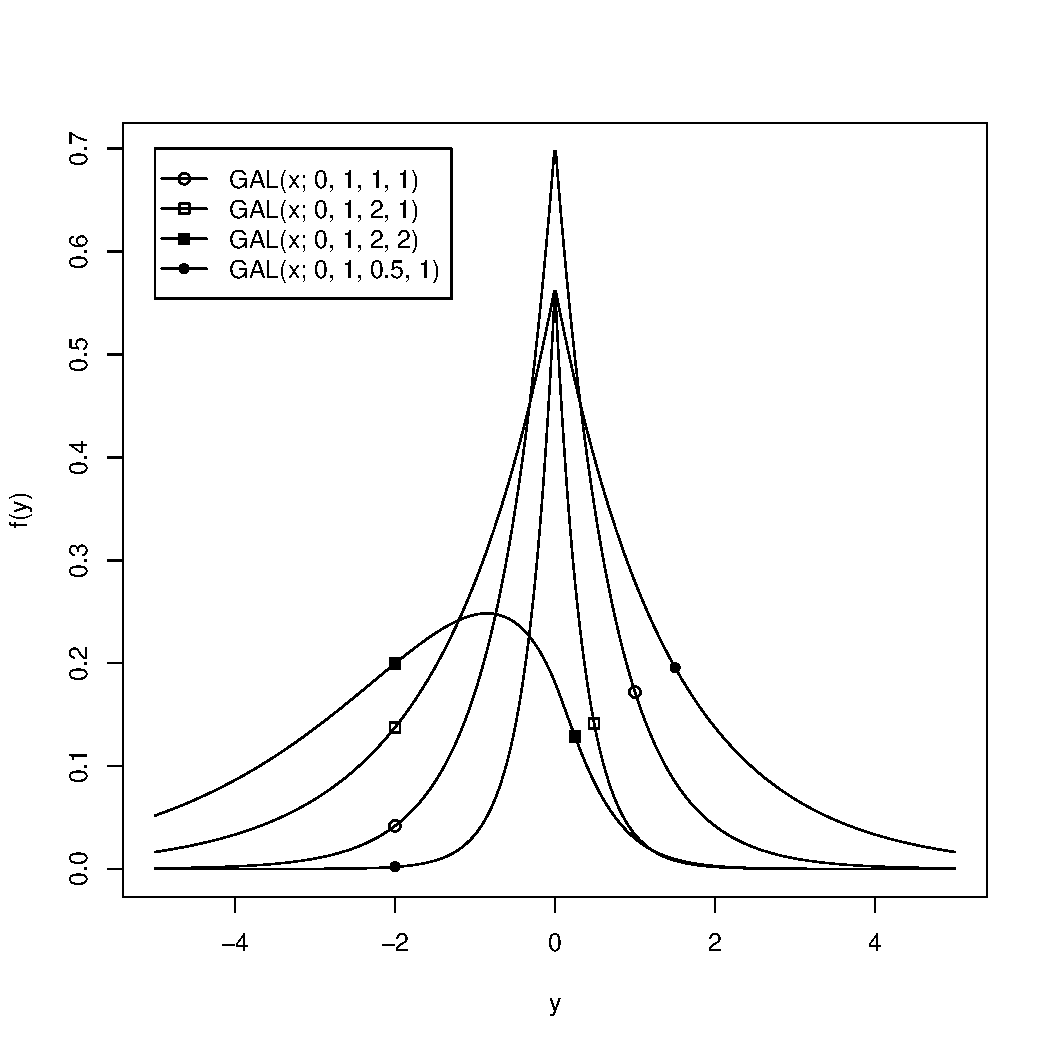
\includegraphics[scale=0.8]{../graphiques/dGAL-exemples.pdf}
  \caption{Fonction de densité de la distribution Laplace asymétrique
    généralisée avec différents paramètres:
    $GAL(y;\theta,\sigma,\kappa,\tau)$}
  \label{fig:densiteGAL}
\end{figure}

Afin de comparer la distribution de Laplace asymétrique généralisée
avec la normale, que l'on cherche à remplacer dans le contexte des
rendements financiers, le comportement des coefficients d'asymétrie
$\gamma_1$ et d'aplatissement $\gamma_2$ de celle-ci peut être
intéressant à observer. On obtient ces derniers à partir des moments
centraux \eqref{eq:momentsGAL} :
\begin{subequations}\label{eq:moments56GAL}
  \begin{align}
    \gamma_1(Y) &= \frac{m_3}{(m_2)^{3/2}} =
    \frac{2\,{\mu}^{3}+3\,{\sigma}^{2}\,\mu}{{\left( {\mu}^{2}+{\sigma}^{2}\right) }^{3/2}\,\sqrt{\tau}}\label{eq:moments5GAL}\\
    \gamma_2(Y) &= \frac{m_4}{(m_2)^{2}} - 3 = \frac{\left(
        3\,{\mu}^{4}+6\,{\sigma}^{2}\,{\mu}^{2}+3\,{\sigma}^{4}\right)
      \,{\tau}^{2}+\left(
        6\,{\mu}^{4}+12\,{\sigma}^{2}\,{\mu}^{2}+3\,{\sigma}^{4}\right)
      \,\tau}{{\left( {\mu}^{2}+{\sigma}^{2}\right) }^{2}\,{\tau}^{2}}
    - 3.\label{eq:moments6GAL}
  \end{align}
\end{subequations}

Le coefficient d'asymétrie de la normale vaut $\gamma_1^N(Y)=0$ et
celui d'excès d'aplatissement, $\gamma_2^N(Y)=0$, puisqu'il a été
défini à partir de cette distribution. Si l'on fixe tous les
paramètres sauf $\mu$, la valeur minimale du coefficient d'excès
d'aplatissement $\gamma_2(Y)$ est atteinte lorsque $\mu$ est de 0:
\begin{align*}
  \min_{\mu} \gamma_2(Y) &= \left[\gamma_2(Y)\right]_{\mu=0} \\
  &= \frac{3}{\tau}.
\end{align*}
Étant donné que le paramètre $\tau$ est strictement positif, la valeur
minimale que peut prendre le coefficient d'excès d'aplatissement
$\gamma_2(Y)$ est plus grande que 0. Par conséquent, l'aplatissement de la
distribution de Laplace asymétrique généralisée sera toujours
supérieur à celui de la normale; c'est donc une distribution
leptocurtique, ce qui est une propriété désirable selon les
observations de \cite{madan1990variance}.

\subsection{Changement d'échelle et de localisation}
\label{sec:transGAL}

Parfois, on doit modifier un ensemble de données afin d'effectuer des
comparaisons ou pour bénéficier des avantages d'une méthode
numérique. Les principales transformations utilisées sont:
\begin{enumerate}
\item un changement de localisation, où l'on additionne une constante
  à l'ensemble des données
\item un changement d'échelle, où l'on multiplie l'ensemble des
  données par un facteur
\item une combinaison des deux transformations précédentes.
\end{enumerate}

Soit deux constantes $a$, $b\neq0$ et une variable aléatoire $X$ qui
suit une distribution Laplace asymétrique généralisée: $X \sim
GAL(\theta,\sigma,\kappa,\tau)$. $Y$ correspond à la somme:
\begin{itemize}
\item de la constante $b$ et
\item du produit:
  \begin{itemize}
  \item de la constante $a$ et
  \item de la variable aléatoire $X$.
  \end{itemize}
\end{itemize}

Selon \cite{kotz2001laplace}, en utilisant le paramètre $\kappa$, on
peut effectuer un changement d'échelle et de localisation et obtenir
une variable aléatoire qui suit encore cette distribution:
\begin{itemize}
\item le paramètre de localisation $\theta$ subit la même
  transformation que la variable aléatoire $X$;
\item le paramètre d'échelle $\sigma$ est multiplié par la constante
  $a$;
\item le paramètre $\kappa$ est inversé si cette constante est
  négative. Ce dernier cas est en fait une réflexion de la
  distribution autour du mode.
\end{itemize}

On a donc:
\begin{align}
  \label{eq:GALscaletrans}
  Y = aX + b \sim GAL(a \theta + b,a\sigma,\kappa^{\sgn{a}\cdot
    1},\tau).
\end{align}

On estime les paramètres $\hat\theta, \hat\sigma, \hat\mu$ et
$\hat\tau$ sur un ensemble de données centrées et réduites $X_t$ à
partir d'un échantillon original $Y_t$. $\hat{m} \text{ et }
\hat{s}>0$ sont respectivement la moyenne et l'écart-type de
l'échantillon $Y_t$. En utilisant l'équation de transformation
\eqref{eq:GALscaletrans} avec les paramètres estimés précédemment, on
peut alors obtenir ceux correspondants pour l'échantillon:
\begin{align}
  \label{eq:transparamGALNS}
  Y_t = \hat{s} X_t + \hat{m} \sim GAL(\hat{s} \theta +
  \hat{m},\hat{s}\sigma,\kappa,\tau) .
\end{align}

Le paramètre $\kappa$ n'est pas modifié puisque l'écart-type $\hat{s}$
est strictement positif. Cette propriété permettra de pratiquer
l'estimation sur des données centrées et réduites, ce qui diminue le
risque d'erreurs numériques sans nuire à sa précision, puisqu'aucune
information contenue dans l'échantillon n'est perdue.

\subsection{Représentation alternative et simulation}
\label{sec:simulationGAL}

Le processus de Laplace $Y(t;\theta,\sigma,\kappa,\tau)$ peut être
représenté sous la forme d'une différence de deux processus gamma
$G_1(t;\tau) - G_2(t;\tau)$ à laquelle on additionne une composante de
dérive. Le premier processus compte les gains, alors que le second,
les pertes. Les deux ont des incréments qui suivent une distribution
gamma $\Gamma(\alpha=\tau, \beta=1)$, c'est-à-dire la même
distribution que le processus
subordonnant utilisé à la section \ref{sec:browniensub}:
\begin{align}
  \label{eq:distributiongammaformealt}
  G_i(\tau) \sim \Gamma\left(\tau,\beta=1 \right), \qquad i\in\left\{
    1,2 \right\}.
\end{align}

Il peut être représenté sous la forme du processus composé suivant:
\begin{align}
  \label{eq:processuslaplace2gamma}
  Y(t) \stackrel{d}{=} \theta +
  \frac{\sigma\sqrt{2}}{2}\left(\frac{1}{\kappa} G_1(t) - \kappa
    G_2(t)\right).
\end{align}

La distribution de Laplace asymétrique généralisée peut alors être
représentée sous la forme d'un incrément de ce processus. Les
variables aléatoires $G_1$ et $G_2$ sont respectivement des
réalisations indépendantes de distribution gamma avec densité
\eqref{eq:densitegamma1}:
\begin{align}
  \label{eq:differencegamma}
  Y \stackrel{d}{=} \theta + \frac{\sigma\sqrt{2}}{2} \left(
    \frac{1}{\kappa} G_1 - \kappa G_2 \right).
\end{align}

Simuler une réalisation de chacune d'entre elles suffira pour obtenir
une réalisation de la distribution gamma. On peut aussi réécrire la
définition précédente de la variable aléatoire $Y$
\eqref{eq:differencegamma} sous la forme simplifiée suivante:
\begin{align}
  \label{eq:differencegamma2}
  Y \stackrel{d}{=} \theta + \left(G_3-G_4 \right).
\end{align}

Les deux variables aléatoires sont alors définies comme suit:
\begin{align*}
  G_3 \sim \Gamma\left(\tau,\beta=\frac{\sqrt{2}}{\kappa\sigma} \right)\\
  G_4 \sim \Gamma\left(\tau,\beta=\frac{\kappa\sigma}{\sqrt{2}}
  \right).
\end{align*}

On peut facilement démontrer l'équivalence en distribution
\eqref{eq:differencegamma2}. En effectuant le produit des fonctions
caractéristiques respectives $\phi_{Y}(\xi)$, $\phi_{G_3}(\xi)$ et
$\phi_{G_4}(\xi)$ des variables aléatoires $Y$, $G_3$ et $G_4$, on
retrouve celle de la forme en $\kappa$:
\begin{align}
  \label{eq:equivalence2gammaFC}
  \phi_{Y}(\xi) &= e^{i\xi\theta} \cdot \phi_{G_3}(\xi) \cdot \phi_{G_4}(\xi) \nonumber\\
  &= e^{i\xi\theta} \cdot \left(\frac{1}{1+i\xi\cdot\frac{\kappa\sigma}{\sqrt{2}}}\right)^{\tau} \cdot \left(\frac{1}{1-i\xi\cdot\frac{\kappa\sigma}{\sqrt{2}}}\right)^{\tau} \nonumber\\
  &=
  \frac{e^{i\xi\theta}}{\left(1-i\xi\frac{\sigma}{\sqrt{2}}\left(\frac{1}{\kappa}-\kappa
      \right) + \frac{\sigma^2\xi^2}{2}\right)^{\tau}}.
\end{align}

La figure \ref{fig:simulGAL} présente un histogramme et un estimateur
de densité par noyau d'un échantillon de 2500 réalisations de la
variable aléatoire $Y$, suivant une distribution de Laplace
asymétrique généralisée de paramètres $\theta=0$, $\sigma=1$,
$\kappa=2$ et $\tau=1$. On remarquera que le paramètre $\kappa$
produit une distribution asymétrique à gauche puisqu'il prend une
valeur supérieure à 1.

\begin{figure}[!ht]
  \centering
  \includegraphics[scale=0.8]{"../graphiques/CH3-SIMULGAL0121"}
  \caption{Histogramme et estimateur de densité par noyau de 2500
    réalisations de la variable aléatoire $Y\sim
    GAL(\theta=0,\sigma=1,\kappa=2,\tau=1)$}
  \label{fig:simulGAL}
\end{figure}

\subsection{Fonction de Bessel et densité}
\label{sec:besseldensiteGAL}

La densité de la distribution Laplace asymétrique généralisée peut
être exprimée à l'aide de la fonction de Bessel modifiée du troisième
type \citep{abramowitz1965handbook}:
\begin{align}
  \label{eq:BesselK}
  K_{\lambda}(u) =
  \frac{(u/2)^{\lambda}\Gamma(1/2)}{\Gamma(\lambda+1/2)}
  \int_1^{\infty} e^{-ut} (t^2-1)^{\lambda-1/2}dt,\qquad \lambda \geq
  -1/2.
\end{align}

On définit les paramètres $\delta = \mu\sigma^{-1}$ et $\eta =
\sqrt{1+\delta^2}$ afin de simplifier la notation.  La démonstration
qui permet d'obtenir la fonction de densité est fondée sur la
définition de la distribution utilisant la différence de deux
processus gamma \eqref{eq:differencegamma}.  Elle est développée par
\cite{kozubowski1999class}:
\begin{align}
  \label{eq:densitekotz}
  f(x) &= \frac{e^{-\kappa^{\sgn(x)}|x|}}{\Gamma(\tau)} \int_{0}^{\infty} y^{\tau-1}(|x|+y)^{\tau-1}e^{-\eta y} dy \nonumber\\
  &= \frac{1}{\Gamma(\tau)\sqrt{\pi}} \left(\frac{|x|}{\eta}
  \right)^{\tau-1/2} e^{\delta x/2} K_{\tau-1/2}\left(\frac{\eta
      |x|}{2}\right).
\end{align}

Afin d'incorporer le paramètre de localisation $\theta$, on remplace
$x$ par la valeur centrée $x-\theta$, et les paramètres $\eta$ et
$\delta$ par ceux d'origine, tels que définis précédemment, pour
obtenir la forme suivante \citep{kotz2001laplace}:
\begin{align}
  \label{eq:densitekotz2001}
  f(x) =
  \frac{\sqrt{2}e^{\frac{\sqrt{2}}{2\sigma}(1/\kappa-\kappa)(x-\theta)}}{\sqrt{\pi}\sigma^{\tau+1/2}\Gamma(\tau)}
  \bigg(\frac{\sqrt{2}|x-\theta|}{\kappa+1/\kappa} \bigg)^{\tau-1/2}
  K_{\tau-1/2}\left(\frac{\sqrt{2}}{2\sigma}\left(\frac{1}{k}+\kappa
    \right)|x-\theta| \right).
\end{align}

Cette fonction a été implémentée dans un algorithme de maximum de
vraisemblance pour le logiciel GNU R par
\cite{RpackageVarianceGamma}. Elle reste cependant sensible
numériquement en plus de demander un temps de calcul important pour de
grands échantillons. De plus, comme la fonction de densité n'est pas
différentiable, on ne peut pas obtenir les estimateurs du maximum de
vraisemblance et leurs matrices de variance-covariance. Donc,
il est impossible d'effectuer de tests d'adéquation ou d'hypothèse avec ces
résultats. C'est une des principales raisons qui ont motivé la
recherche d'autres méthodes d'estimation plus efficaces pour cette
distribution.

\section{Cas particuliers}
\label{sec:cas-particuliers}

La distribution de Laplace asymétrique généralisée peut être
considérée comme une extension de plusieurs cas particuliers. Ces
distributions ainsi que leur notation et leur fonction de densité sont
présentées dans la table \ref{tab:casspeciauxGAL}.
\begin{table}[!ht]
  \centering
  \begin{tabular}{cccc}
    \hline
    \textbf{Cas} & \textbf{Distribution} & \textbf{Notation} & \textbf{Densité} \\
    \hline
    $\theta=0$ & \multirow{4}{*}{Exponentielle de moyenne $\mu>0$} & \multirow{4}{*}{$GAL(0,0,\mu,1)$} & \multirow{4}{*}{$\frac{1}{\mu}e^{-x/\mu}\,(x > 0)$} \\ 
    $\sigma=0$ &  &  &  \\
    $\mu>0$ &  &  &  \\ 
    $\tau=1$ &  &  &  \\ \hline
    $\theta=0$ & \multirow{3}{*}{Gamma de paramètres $\alpha=\tau$, $\beta=\mu>0$} &
    \multirow{3}{*}{$GAL(0,0,\mu,\tau)$} & \multirow{3}{*}{$\frac{x^{\tau-1}e^{-x/\mu}}{\mu^\tau\Gamma(\tau)},(x > 0)$} \\
    $\sigma=0$ &  &  &  \\
    $\mu>0$ &  &  &  \\ \hline
    $\sigma>0$ & \multirow{3}{*}{Laplace symétrique $(\sigma>0)$} &
    \multirow{3}{*}{$GAL(\theta,\sigma,0,1)$} & \multirow{3}{*}{$\frac{1}{\sqrt{2}\sigma}e^{-\sqrt{2}|x-\theta|/\sigma},(x \in \mathbb{R})$} \\
    $\mu=0$ &  &  &  \\
    $\tau=1$ &  &  &  \\ \hline
    $\sigma>0$ & \multirow{3}{*}{Laplace asymétrique $(\sigma>0)$} &
    \multirow{3}{*}{$GAL(\theta,\sigma,\mu,1)$} & \multirow{3}{*}{$\frac{\sqrt{2}\kappa}{\sigma(1+\kappa^2)}\begin{cases}e^{\frac{\sqrt{2}\kappa}{\sigma}(\theta-x)},\quad & x\geq\theta \\ e^{\frac{\sqrt{2}}{\sigma\kappa}(x-\theta)},\quad & x < \theta \end{cases}$} \\
    $\mu \neq 0$ &  &  &  \\
    $\tau=1$ &  &  &  \\ \hline
    $\sigma=0$ & \multirow{3}{*}{Dégénérée à $\theta$} & \multirow{3}{*}{$GAL(\theta,0,0,0)$} & \multirow{3}{*}{$1_{x=\theta}$} \\
    $\mu=0$ &  &  &  \\ 
    $\tau=0$ &  &  &  \\ \hline
  \end{tabular}
  \caption{Cas spéciaux de la distribution de Laplace asymétrique généralisée}
  \label{tab:casspeciauxGAL}
\end{table}

Les deux premiers cas spéciaux sont des distributions de probabilité
classiques. L’attention sera portée sur la distribution de Laplace
asymétrique et son cas spécial, celle de Laplace symétrique. La
dégénérée n'a aucune application pratique, mais en mentionner
l'existence est pertinent, puisque ce ne sont pas toutes les
distributions qui admettent ce cas.

\subsection{Distribution de Laplace asymétrique}
\label{sec:distributionAL}

La distribution de Laplace asymétrique a été introduite
par \cite{hinkley1977estimation} et étudiée en profondeur par
\cite{kozubowski1999class}.  Cette distribution a elle aussi plusieurs
caractéristiques intéressantes pour remplacer la normale, dans le
contexte de la modélisation financière, comme le présentent
\cite{kozubowski2001asymmetric}. Elle est notée
$AL(\theta,\sigma,\kappa)$.

Cette distribution, en tant que cas particulier de la distribution de
Laplace asymétrique généralisée, conserve la majorité de ses
propriétés.  Entre autres, elle est infiniment divisible et possède des moments
finis. Les paramètres $\theta$, $\sigma$ et $\kappa$ conservent leurs
rôles et propriétés définis à la section \ref{sec:momentsGAL}. On peut
donc contrôler la localisation, l'échelle et l'asymétrie de la
distribution. Cependant, aucun paramètre ne permet de contrôler le
coefficient d'aplatissement.

La densité de probabilité de cette distribution
$f(x;\theta,\sigma,\kappa)$ présente une forme analytique simple qui
ne requiert pas le recours à la fonction de Bessel modifiée de
troisième type \eqref{eq:BesselK}.
\begin{align}
  \label{eq:densiteAL}
  f(x;\theta,\sigma,\kappa) =
  \frac{\sqrt{2}}{\sigma}\frac{\kappa}{1+\kappa^2} \begin{cases}
    \exp\left(\frac{-\sqrt{2}\kappa}{\sigma}\left( x-\theta \right)\right),\quad & x\geq\theta \\
    \exp\left( \frac{\sqrt{2}}{\theta\kappa}\left(\theta - x \right)
    \right),\quad & x<\theta.\end{cases}
\end{align}

La fonction caractéristique de cette distribution prend la forme
suivante:
\begin{align}
  \label{eq:caractALkappa}
  \phi(t;\theta,\sigma,\kappa) = \frac{e^{i \theta
      t}}{1+\frac{\sigma^2 t^2}{2}-
    i\frac{\sigma}{\sqrt{2}}\left(\frac{1}{\kappa}-\kappa \right)
    t}\,.
\end{align}

Cette dernière est utilisée principalement lorsque l'application d'une
propriété nécessite une distribution avec un seul paramètre d'échelle.
La seconde paramétrisation de cette distribution utilise le paramètre
$\mu$ qui n'est pas invariant d'échelle.  Cette paramétrisation donne
une forme beaucoup plus simple de la fonction caractéristique
\eqref{eq:caractALkappa}:
\begin{align}
  \label{eq:caractALmu}
  \phi(t\theta,\sigma,\mu) = \frac{e^{i \theta t}}{1+\frac{\sigma^2
      t^2}{2}- i\mu t}.
\end{align}

On reconnait la fonction caractéristique d'un incrément du processus
de Laplace \eqref{eq:fncaractprocessuslaplace} avec les paramètres
($\tau=1$, $t=1$). Une forme standardisée de cette distribution existe
aussi avec le paramètre d'échelle $\sigma=1$ et de dérive $\theta=0$.
Enfin, on peut avoir une représentation alternative de cette
distribution, utilisée principalement pour la simulation, basée sur
l'exponentielle:
\begin{align}
  \label{eq:ALrepsimul}
  Y &= \theta + \frac{\sigma}{\sqrt{2}} \left(\frac{1}{\kappa}W_1 - k W_2 \right)
\end{align}
où
\begin{align*}
  W_1 \sim \mbox{Exponentielle}\left(\frac{\sigma}{\sqrt{2}\kappa}\right) \nonumber \mbox{ et } W_2 \sim \mbox{Exponentielle}\left(\frac{\sigma\kappa}{\sqrt{2}}\right)
\end{align*}

Cette méthode n'est cependant pas la plus efficace pour simuler une
réalisation $Y$ de la distribution de Laplace asymétrique, car on peut
la faire à partir de deux réalisations indépendantes $U_1$ et $U_2 $
d'une variable aléatoire uniforme définie sur l'intervalle
$\left[0,1\right]$:
\begin{align}
  \label{eq:simulALunif}
  Y = \theta + \frac{\sigma}{\sqrt{2}}
  \ln{\frac{U_1^\kappa}{U_2^{1/\kappa}}}.
\end{align}

Lorsque le paramètre $\tau$ de la distribution de Laplace asymétrique
généralisée est un entier, on peut générer une réalisation $X$ de
celle-ci en sommant un total de $\tau$ réalisations indépendantes de
la variable aléatoire $Y$:
\begin{align*}
  X &= \sum_{i=1}^{\tau} Y_{i} \\
  Y_{i} &\sim AL(\theta,\sigma,\kappa).
\end{align*}

\section{Relation avec le modèle de \cite{madan1990variance}}
\label{sec:relation-avec-le}

Le modèle Variance Gamma de \cite{madan1990variance} utilise une
paramétrisation différente de celle de \cite{kotz2001laplace}. On
doit, afin de conserver une compatibilité des développements des
prochains chapitres, détailler les changements de paramètres qui
permettent de passer d'un modèle à l'autre. Le modèle Variance Gamma
utilise les paramètres $C,\sigma,\theta \mbox{ et } \nu$. Afin
d'éviter la confusion, les paramètres seront indicés de 1 à 3 selon le
modèle d'où ils proviennent. Le modèle 1 sera celui de
\cite{madan1990variance}, les modèles 2 et 3 seront respectivement les
paramétrisations en $\mu$ et en $\kappa$ de
\cite{kotz2001laplace}. Les différentes équivalences se trouvent à la
table \ref{tab:chparam}.
\begin{table}[!ht]
  \centering
  \begin{tabular}{cccccc}
    \hline
    \textbf{Vers le modèle} & &  & \textbf{À partir du modèle} &  & \textbf{À partir du modèle} \\ \hline
    \textbf{1} & &  & \textbf{2} &  & \textbf{3} \\ \hline
    
    & $C$ & $=$ & $\theta_2$ & $=$ & $\theta_3$ \\ 
    \multicolumn{ 1}{l}{} & $\sigma_1$ & $=$ & $\sqrt{\tau_2}\sigma_2$ & $=$ & $\sqrt{\tau_3}\sigma_3$ \\ 
    \multicolumn{ 1}{l}{} & $\theta_1$ & $=$ & $\mu\tau_2$ & $=$ & $\tau_3\sigma_3(1/\kappa - \kappa)/\sqrt{2}$ \\ 
    \multicolumn{ 1}{l}{} & $\nu$ & $=$ & $1/\tau_2$ & $=$ & $1/\tau_3$ \\ 
    \hline
    \textbf{2} & &  & \textbf{1} &  & \textbf{3} \\ \hline
    & $\theta_2$ & $=$ & $C$ & $=$ & $\theta_3$ \\ 
    \multicolumn{ 1}{l}{} & $\sigma_2$ & $=$ & $\sigma_1\sqrt{\nu}$ & $=$ & $\sigma_3$ \\ 
    \multicolumn{ 1}{l}{} & $\mu$ & $=$ & $\theta_1*\nu$ & $=$ & $\sigma_3(1/\kappa - \kappa)/\sqrt{2}$ \\ 
    \multicolumn{ 1}{l}{} & $\tau_2$ & $=$ & $1/\nu$ & $=$ & $\tau_3$ \\ 
    \hline
    \textbf{3} & &  & \textbf{1} &  & \textbf{2} \\ \hline
    & $\theta_3$ & $=$ & $C$ & $=$ & $\theta_2$ \\ 
    \multicolumn{ 1}{l}{} & $\sigma_3$ & $=$ & $\sigma_1\sqrt{\nu}$ & $=$ & $\sigma_2$ \\ 
    \multicolumn{ 1}{l}{} & $\kappa$ & $=$ & $\frac{\sqrt{2(\sigma_1\sqrt{\nu})^2 + (\theta_1*\nu)^2} – \theta_1*\nu}{\sigma_1\sqrt{\nu}\sqrt{2}}$ & $=$ & $\frac{\sqrt{2(\sigma_2)^2 + \mu^2} - \mu}{\sigma_2\sqrt{2}}$ \\ 
    \multicolumn{ 1}{l}{} & $\tau_3$ & $=$ & $1/\nu$ & $=$ & $\tau_2$ \\ \hline
  \end{tabular}
  \caption{Changements de paramétrisation}
  \label{tab:chparam}
\end{table}



%%% Local Variables: 
%%% mode: latex
%%% TeX-master: "gabarit-maitrise"
%%% End: 

             % chapitre 2, etc.
\chapter*{Conclusion} % ne pas numéroter
\phantomsection\addcontentsline{toc}{chapter}{Conclusion} % dans TdM

%% Revenir sur le papier de Derman, résumé des avantages et
%% inconvénients du modèle, des méthodes d'estimation et d'évaluation
%% d'options

En guise de conclusion, j'aimerais tout d'abord effectuer un retour
sur les différents éléments introduits au début du premier chapitre,
concernant le risque de modélisation. Le modèle présenté n'en est pas
exempt, bien au contraire. Cependant, il
nécessite moins d'hypothèses restrictives que les autres modèles
présentés pour être valide, bien qu'il exige toujours l'indépendance
des observations. Il tient compte de la possibilité de sauts tout en
conservant une composante de mouvement aléatoire, ce qui décrit
adéquatement les observations empiriques à ce jour. Comme tout modèle
paramétrique, il reste dépendant du nombre et de la qualité des
données disponibles. Étant donné que l'utilisation d'algorithmes
d'optimisation numérique est inévitable, il subsiste un risque
important autour de l'estimation des paramètres et de l'approximation de la distribution. De plus, étant donné qu'il n'existe pas
de mesure neutre au risque unique, l'arbitrage de modèle reste
possible et doit être considéré. L'utilisation d'un échantillon de
données instables à travers le temps peut produire des résultats
inattendus, surtout au niveau de la distribution de la volatilité
historique, un aspect qui pourra être approfondi ultérieurement.
Enfin, subsiste toujours le risque d'erreurs de nature informatique
qui pourraient produire de faux résultats.

Ce retour permet de constater qu'il y a toujours place à
l'amélioration des outils développés. Entre autres, il pourrait être
pertinent d'étudier les différences entre le comportement à court et à long terme du modèle. En se basant sur la théorie de
l'utilité, on pourrait développer une meilleure approche pour
déterminer les paramètres de la distribution neutre au risque. Il
pourrait aussi être intéressant de développer des mesures de risque
cohérentes pour les processus de Lévy, notamment
avec les avancées de celles basées sur l'entropie. L'extension
multivariée de ce modèle n'a toujours pas été développée dans la
littérature, alors il pourrait être pertinent de s'y attarder, entre
autres pour étudier les titres indiciels et optimiser la composition
de portefeuilles. Enfin, il pourrait être intéressant d'aborder le
problème inverse de l'estimation des paramètres à partir des prix des
produits dérivés observés sur les marchés financiers.

%%% Local Variables: 
%%% mode: latex
%%% TeX-master: "gabarit-maitrise"
%%% End: 
            % conclusion

\appendix                       % annexes le cas échéant

\include{annexe}                % annexe A

\bibliography{}                 % production de la bibliographie

\end{document}
%</gabarit>
%
% ^^A Gabarits des parties du document
%<*resume>
\chapter*{Résumé}                      % ne pas numéroter
\phantomsection\addcontentsline{toc}{chapter}{Résumé} % inclure dans TdM

\begin{otherlanguage*}{francais}
  Texte du résumé en français.
\end{otherlanguage*}
%</resume>
%
%<*abstract>
\chapter*{Abstract}                      % ne pas numéroter
\phantomsection\addcontentsline{toc}{chapter}{Abstract} % inclure dans TdM

\begin{otherlanguage*}{english}
  Text of English abstract.
\end{otherlanguage*}
%</abstract>
%
%<*remerciements>
\chapter*{Remerciements}         % ne pas numéroter
\phantomsection\addcontentsline{toc}{chapter}{Remerciements} % inclure dans TdM

Texte des remerciements en prose.
%</remerciements>
%
%<*avantpropos>
\chapter*{Avant-propos}         % ne pas numéroter
\phantomsection\addcontentsline{toc}{chapter}{Avant-propos} % inclure dans TdM

L'avant-propos est surtout nécessaire pour une thèse par article.
%</avantpropos>
%
%<*introduction>
\chapter*{Introduction}         % ne pas numéroter
\phantomsection\addcontentsline{toc}{chapter}{Introduction} % inclure dans TdM

Une thèse ou un mémoire devrait normalement débuter par une
introduction. Celle-ci est traitée comme un chapitre normal, sauf
qu'elle n'est pas numérotée.
%</introduction>
%
%<*chapitre>
\chapter{Titre du chapitre}     % numéroté

Texte du chapitre.
%</chapitre>
%
%<*conclusion>
\chapter*{Conclusion}         % ne pas numéroter
\phantomsection\addcontentsline{toc}{chapter}{Conclusion} % dans TdM

Une thèse ou un mémoire devrait normalement se terminer par une
conclusion, placée avant les annexes, le cas échéant. Celle-ci est
traitée comme un chapitre normal, sauf qu'elle n'est pas numérotée.
%</conclusion>
%
%<*annexe>
\chapter{Titre de l'annexe}     % numérotée

Texte de l'annexe.
%</annexe>
% Local Variables:
% mode: doctex
% coding: utf-8
% TeX-master: t
% End:
% \fi
